
\chapter{SOCIOLINGUISTIQUE : LA PRISE EN COMPTE DE L’EXTRALINGUISTIQUE}
\label{chapter-13}
\markright{Sociolinguistique}
\origpage{388}{374}
\begin{keybox}[Plan du chapitre]
\small\setstretch{1.01}
\setlist{topsep=.12em,itemsep=.12em,parsep=0pt}
\textbf{I.\quad LA LINGUISTIQUE VARIATIONNISTE}
\begin{enumerate}[label=\arabic*.]
\item William Labov : le pionnier\par \textcircled{\scriptsize 1} Apport scientifique et méthodologique\par \textcircled{\scriptsize 2} L’expérience à Martha’s Vineyard\par \textcircled{\scriptsize 3} L’expérience à New York City\par\hspace*{1em}1. L’hypercorrection\par\hspace*{1em}2. L’hypocorrection
\item La variation linguistique\par \textcircled{\scriptsize 1} La variation diachronique\par \textcircled{\scriptsize 2} La variation diatopique\par \textcircled{\scriptsize 3} La variation diastratique\par \textcircled{\scriptsize 4} La variation diaphasique\par \textcircled{\scriptsize 5} La variation diamésique
\item Le schibboleth, révélateur d’appartenance linguistique\ednote{章首提纲写 « schibboleth »；正文标题主要用 « shibboleth »。标准拼写通常为 shibboleth，本版依底本保留两种拼写。}\par \textcircled{\scriptsize 1} Origine de la notion\par \textcircled{\scriptsize 2} Le shibboleth social : l’anglais U et Non-U\par\hspace*{1em}1. Origine de la notion\par\hspace*{1em}2. Les effets de démonstration\par\hspace*{1em}3. Répercussions\par \textcircled{\scriptsize 3} Le shibboleth social chez Proust
\end{enumerate}
\textbf{II.\quad PLURILINGUISME ET DIGLOSSIE}
\begin{enumerate}[label=\arabic*.]
\item Multilinguisme et plurilinguisme\par \textcircled{\scriptsize 1} Définition du Conseil de l’Europe\par \textcircled{\scriptsize 2} Déclaration de Salzbourg pour un monde multilingue\par \textcircled{\scriptsize 3} Le degré de maîtrise des langues
\item Typologie du bilinguisme individuel\par \textcircled{\scriptsize 1} Difficultés autour d’une définition\par \textcircled{\scriptsize 2} Bilinguisme individuel et social\par \textcircled{\scriptsize 3} Bilinguisme équilibré et dominant
\tcbbreak\origpage{389}{375}
\textcircled{\scriptsize 4} Bilinguisme composé et coordonné\par \textcircled{\scriptsize 5} Bilinguisme précoce simultané et précoce consécutif\par \textcircled{\scriptsize 6} Bilinguisme additif et soustractif\par \textcircled{\scriptsize 7} Bilingue biculturel et monoculturel
\item L’alternance codique (code-switching)\par \textcircled{\scriptsize 1} Définitions\par \textcircled{\scriptsize 2} Code-switching balisé et code-switching fluide\par \textcircled{\scriptsize 3} Le code-switching interphrastique\par \textcircled{\scriptsize 4} Le code-switching intraphrastique\par \textcircled{\scriptsize 5} Le code-switching extraphrastique
\item Le bilinguisme social : la diglossie\par \textcircled{\scriptsize 1} Bilinguisme et diglossie\par \textcircled{\scriptsize 2} William Marçais : la diglossie arabe\par \textcircled{\scriptsize 3} Charles Albert Ferguson : Diglossia\par \textcircled{\scriptsize 4} Derek Bickerton : basilecte, mésolectes et acrolectes\par \textcircled{\scriptsize 5} La diglossie en France\par\hspace*{1em}1. La diglossie français/latin\par\hspace*{1em}2. La langue des lettres et de l’esprit\par\hspace*{1em}3. La diglossie français/patois\par\hspace*{2em}1) L’abbé Grégoire\par\hspace*{2em}2) Le Rapport Grégoire : l’éradication des patois
\end{enumerate}
\textbf{III.\quad LINGUISTIQUE ET GÉOGRAPHIE : LA DIALECTOLOGIE}
\begin{enumerate}[label=\arabic*.]
\item Objet et méthodes\par \textcircled{\scriptsize 1} Description interne\par \textcircled{\scriptsize 2} Description contrastive\par \textcircled{\scriptsize 3} Description génétique\par \textcircled{\scriptsize 4} Description anthropologique\par \textcircled{\scriptsize 5} Description sociolinguistique
\item Continuum et frontière linguistique\par \textcircled{\scriptsize 1} Exemple de continuum linguistique\par \textcircled{\scriptsize 2} Exemple de frontière linguistique\par \textcircled{\scriptsize 3} Exemple d’isoglosse : la ligne Joret
\end{enumerate}
\textbf{IV.\quad INTERFÉRENCE ENTRE SYSTÈMES LINGUISTIQUES}
\begin{enumerate}[label=\arabic*.]
\item Langues vernaculaires et véhiculaires\par \textcircled{\scriptsize 1} Les langues vernaculaires\par \textcircled{\scriptsize 2} Les langues véhiculaires
\tcbbreak\origpage{390}{376}
\item Les langues de relation\par \textcircled{\scriptsize 1} Le sabir\par \textcircled{\scriptsize 2} La lingua franca\par \textcircled{\scriptsize 3} La koinè
\item Les pidgins\par \textcircled{\scriptsize 1} Le pidgin anglo-chinois（洋泾浜英语）\par\hspace*{1em}1. Contexte d’apparition\par\hspace*{1em}2. Traces dans le chinois moderne\par \textcircled{\scriptsize 2} Le pidgin camerounais : le camfranglais\par\hspace*{1em}1. Contexte d’apparition\par\hspace*{1em}2. Statut linguistique\par \textcircled{\scriptsize 3} Le bichlamar des îles Vanuatu\par\hspace*{1em}1. Contexte d’apparition\par\hspace*{1em}2. Statut linguistique\par\hspace*{1em}3. Lexique en bichlamar
\item Les créoles\par \textcircled{\scriptsize 1} Le processus de créolisation\par \textcircled{\scriptsize 2} Différence entre pidgin et créole\par \textcircled{\scriptsize 3} Exemples de langues créoles\par\hspace*{1em}1. Le tok pisin de Papouasie\par\hspace*{1em}2. Le pijin des îles Salomon\par\hspace*{1em}3. Le patoa de Macao
\end{enumerate}
\textbf{Exercices}\par\textbf{Pour aller plus loin}\par\textbf{Glossaire}
\end{keybox}

\origpage{391}{377}
\begin{keybox}[Introduction]
La sociolinguistique est née dans les années 1960 aux États-Unis autour d’un groupe de chercheurs dont les plus connus sont Dell Hymes, Joshua Fishman, John Gumperz, Charles Ferguson et William Labov. Pour Fishman, cette branche de la linguistique consiste à : « Étudier qui parle quoi, comment où et à qui ». La sociolinguistique, comme la pragmatique et la linguistique de l’énonciation, s’oppose à la tradition saussurienne et aux enseignements du \textit{Cours de linguistique générale}. William Labov fait aux linguistes saussuriens le reproche suivant :
\begin{quote}
Ils s’obstinent à rendre compte des faits linguistiques par d’autres faits linguistiques, et refusent toute explication fondée sur des données extérieures tirées du comportement social [...] La sociolinguistique prend en compte tous les phénomènes liés à l’homme parlant au sein d’une société.
\end{quote}
La sociolinguistique est donc née d’une critique des orientations théoriques et méthodologiques de la linguistique structurale immanente qui étudie la langue indépendamment de la réalité extralinguistique. Pour cette raison, certains linguistes ont parlé d’une linguistique en crise incapable d’intégrer de manière satisfaisante la notion de variation et de répondre aux questions liées à la place et au rôle des phénomènes langagiers dans la société. La linguistique moderne, la sociolinguistique et la géolinguistique en particulier, ont réintégré les facteurs externes dans la réflexion sur le langage, à savoir les facteurs sociaux et géographiques.
\end{keybox}

\section{LA LINGUISTIQUE VARIATIONNISTE}
Dans le chapitre précédent, nous avons vu qu’à travers le choix de la parole comme objet d’étude, la linguistique de l’énonciation et la pragmatique ont réintégré le locuteur dans le champ de la réflexion sur le langage. Dans ce chapitre, avec la sociolinguistique, c’est sur la communauté linguistique, que Saussure appelait les « masses parlantes », que se porte le focus. C’est cette communauté qui est en partie responsable de la « mutabilité du signe » et donc de la variation linguistique.

\subsection{William Labov : le pionnier}
Linguiste américain \textbf{William Labov} (1927-) est considéré comme l’un des fondateurs de la sociolinguistique moderne. Plus précisément, il est, avec \textbf{Uriel Weinreich} (1926-1967), un des pères de la linguistique « variationniste » qui considère le langage comme sujet à la variabilité tout en étant ordonné dans son hétérogénéité. Labov a toujours reconnu l’influence d’Uriel Weinreich sur le développement de ses idées, sous la direction de qui À l’Université de Columbia il a rédigé sa thèse de\origfoot{1}{Joshua Fishman, \textit{Sociolinguistique}, Nathan, Paris, 1971.}\ednote{原文 « sous la direction de qui À l’Université de Columbia » 句法与大小写均有问题；较自然的表述应为 « sous la direction de qui, à l’Université de Columbia, il a rédigé… » 或改用 « sous la direction duquel »。正文依底本保留。}
\origpage{392}{378}
doctorat : \textit{The social stratification of English in New York City Department Stores}. Posant un regard critique sur certaines démarches scientifiques auxquelles les linguistes avaient alors fréquemment recours, notamment l’introspection et les jugements \textit{a priori}, il a proposé une nouvelle manière de faire de la linguistique :

\begin{lecture}{Extrait}
La plupart des linguistes rassemblent des données en procédant par introspection, en se demandant : Est-ce que je peux dire ceci ? Est-ce que je peux dire cela ? J’ai donc pensé que je pourrais initier une nouvelle manière de faire de la linguistique en basant l’étude du langage sur ce les les gens\ednote{原文 « sur ce les les gens »；语法上显然缺 que 且多出一个 les，应为 « sur ce que les gens »。} disent réellement dans la vraie vie quotidienne.
\end{lecture}

\minititle{\textcircled{\scriptsize 1} Apport scientifique et méthodologique}
William Labov a été le premier à développer une étude de la variation dotée d’outils descriptifs véritablement performants, à base de description quantitative et de modèles théoriques. Selon lui, la sociolinguistique doit être en mesure d’expliquer et de décrire les variations dans l’usage de la langue, tant à l’échelle microsociale (au niveau de l’individu et des relations interindividuelles) qu’à l’échelle macrosociale (au niveau d’une communauté entière). Labov s’oppose aussi à la grammaire générative et à la linguistique chomskyenne (objet du prochain chapitre) qui étudie la norme linguistique sans tenir compte de l’usage. Enfin, la sociolinguistique a pour mission de montrer que la variation n’est pas libre, mais structurée par des règles sous-jacentes. Selon lui, le processus du changement se déroule en trois étapes. Dans un premier temps, le changement concerne une variation dans le discours de quelques personnes. Dans un deuxième temps, il se propage, se développe et s’oppose à l’ancienne forme. Enfin, il s’accomplit et élimine les formes rivales.

\minititle{\textcircled{\scriptsize 2} L’expérience à Martha’s Vineyard}
En 1963, Labov a passé des vacances sur la petite île de Martha’s Vineyard, au large du Massachusetts. Aujourd’hui, Martha’s Vineyard est un lieu de villégiature pour milliardaires et célébrités, mais à l’époque du séjour de Labov, le tourisme ne se développait que depuis peu et Labov a constaté que l’enthousiasme des autochtones à recevoir les vacanciers fortunés venus de la ville variait considérablement d’une personne à l’autre. En particulier, il a noté une variation phonétique typique de l’île dans la prononciation de certains phonèmes, en particulier le /au/ de \textit{mouse} et le /ay/ de \textit{mice}, prononcés d’une manière plus ou moins exagérée selon les habitants. Labov a établi que les habitants favorables au tourisme prononçaient les deux phonèmes de la même manière que les touristes, dans un américain standard. Au contraire, ceux qui s’opposaient au développement du tourisme, parmi lesquels on trouvait les derniers marins de l’île et dont l’activité de pêche était menacée par l’arrivée des touristes, avaient tendance à conserver, voire à exagérer l’accent local, comme une marque de rejet.

\minititle{\textcircled{\scriptsize 3} L’expérience à New York City}
On l’a évoqué en tout début de chapitre : la variation liée à la classe sociale dans la prononciation constitue un centre d’intérêt majeur pour Labov. Une étude fondatrice en la matière est sa thèse de
\origpage{393}{379}
doctorat, consacrée à la prononciation du /r/ à New York, publiée en 1966 sous le titre \textit{The social stratification of English in New York City}. Pour effectuer ses travaux de recherche, Labov s’est rendu dans trois chaînes de magasins de vêtements ciblant des clientèles socialement différentes : Saks Fifth Avenue (enseigne luxueuse), Macy’s (classes moyennes) et S. Klein (classes populaires). Ayant choisi ces magasins de telle sorte qu’à chaque fois, les bas en nylon soient vendus au quatrième étage (\textit{fourth floor}), sa démarche d’investigation a consisté à demander aux clients de ces trois magasins où se trouvaient les bas en nylon, afin de les entendre prononcer « fourth floor ». Son objectif était d’étudier la variation de prononciation du même phonème chez les classes supérieures, moyennes, et populaires. Le résultat de cette enquête a mis en évidence un phénomène d’hypercorrection chez la classe moyenne, dont la production de la variante prestigieuse du /r/ surpassait celle de la classe supérieure. En revanche, chez S. Klein, l’insistance sur la prononciation du /r/ était presque inexistante.

\minititle{1. L’hypercorrection}
L’hypercorrection est un phénomène qui consiste à s’exprimer de manière incorrecte du fait même de vouloir parler le plus correctement possible. Elle apparaît lorsque le locuteur essaie de pallier à son insécurité linguistique\ednote{传统规范语法中 pallier 通常作直接及物动词，写作 « pallier son insécurité linguistique »；正文保留底本 « pallier à »。}. En français par exemple, une manifestation courante de l’hypercorrection se trouve dans les liaisons erronées, non justifiées par l’orthographe : l’énoncé « il va être midi » prononcé [ilvatetw(o)midi], c’est-à-dire « il va-t-être midi », révèle chez le locuteur une volonté de faire les liaisons même lorsque l’orthographe ne le justifie pas. À l’écrit, l’hypercorrection peut prendre la forme d’un ajout d’accents circonflexes (« faîtes comme chez vous »), de « h » étymologiques (« enthropie »), de « s » après une consonne muette (« le camps »), ou de « ç » devant un « i » ou un « e », etc.

Pour le sociologue français \textbf{Pierre Bourdieu} (1930-2002), l’hypercorrection est un phénomène caractéristique du « parler petit-bourgeois », qui révèle, dans une société donnée, l’estime ou la valeur qu’attribuent les locuteurs à certaines règles de langage. La règle de la liaison est, en cela, perçue comme plus importante que la concordance des temps, et les fautes de liaison sont parfois beaucoup plus marquantes que les fautes de temps. L’étude du phénomène d’hypercorrection montre que dans un groupe, un sujet qui s’exprime à l’oral ou à l’écrit fait des choix linguistiques ; qui révèlent sa posture par rapport au groupe.\ednote{原文在 « choix linguistiques ; qui révèlent » 之间用分号切断关系从句；按句法应改为逗号或直接删除分号。} L’hypercorrection ou, à l’inverse, l’hypocorrection, sont des moyens de marquer sa différence au sein du groupe.

\minititle{2. L’hypocorrection}
L’hypocorrection est l’introduction dans un discours d’hésitations (« bon », « alors », « heu »), de formulations incorrectes, ou encore l’utilisation de vocabulaire familier ou peu étendu. Ce phénomène peut être plus ou moins conscient, et s’il est conscient, il fait alors partie de la stratégie de communication du locuteur. Mais il est difficile de distinguer d’une part ce qui doit être attribué à de vraies hésitations, de vraies difficultés dans l’énonciation, et d’autre part ce qui relève d’une volonté de ne pas faire perdre la face à l’interlocuteur, de ne pas l’inquiéter par un discours au registre trop élevé, ou par trop d’assurance pouvant être perçus comme un FTA (\textit{Face Threatening
\origpage{394}{380}
Act}). Sur l’hypocorrection, je vous invite à lire le très beau texte de Marcel Pagnol (1895-1974) dans les exercices de fin de page.

\subsection{La variation linguistique}
Commençons par une évidence : nous ne parlons pas de la même façon dans toutes les circonstances. Au cours d’une journée, nous changeons de variété de langue en fonction de nos interlocuteurs, de l’objet de notre prise de parole, des conditions immédiates d’énonciation, etc. De même, en fonction de notre milieu social, de notre histoire personnelle, de notre implantation géographique, des effets perlocutoires que l’on veut produire sur autrui, de la maîtrise des différents registres de notre langue, nous avons recours à des variétés linguistiques très diverses, qui, même si elles appartiennent à la même langue, peuvent comporter des différences considérables. Pour Labov, l’objet d’étude de la sociolinguistique est « la structure et l’évolution du langage au sein du contexte social formé par la communauté linguistique ». Pour lui, il n’y a pas d’étude de la langue possible sans prise en compte des hommes qui la parlent et sans prise en compte de l’environnement social. Il a donc tenté de corréler les manières de parler avec les variables sociales et d’associer chaque variante linguistique à une cause extralinguistique, comme la classe sociale, le sexe, l’âge, l’habitat, la race, les circonstances de la communication, etc. Il distingue ainsi quatre types de variation.

\minititle{\textcircled{\scriptsize 1} La variation diachronique}
La variation diachronique joue, vous l’avez sûrement deviné, sur l’axe temporel. La variante de langue liée à des conditions temporelles est appelée chronolecte. On ne parle pas aujourd’hui comme à l’époque de Molière, et employer de nos jours des expressions aussi datées que « fichtre ! », « diantre ! », « sacrebleu ! » provoquerait l’incompréhension de nos contemporains.

\minititle{\textcircled{\scriptsize 2} La variation diatopique}
La variation diatopique (du grec \textit{topos}, le lieu) joue sur l’axe géographique. Pour désigner les différents types de variation diatopique, on distingue les géolectes (variétés linguistiques propres à une aire géographique), qui se divisent à leur tour en régiolectes (à l’échelle infranationale) et en topolectes, pour les espaces géographiques limités : village, vallée, quartier, etc.

\minititle{\textcircled{\scriptsize 3} La variation diastratique}
La variation diastratique explique les différences des usages langagiers entre les diverses classes sociales. Envisagée sous l’angle social et démographique (âge, sexe, milieu social, profession, niveau d’étude, ville ou campagne, etc.), on parle de sociolecte. Un jargon, professionnel ou académique, est un genre de sociolecte appelé technolecte.

\minititle{\textcircled{\scriptsize 4} La variation diaphasique}
On parle de variation diaphasique lorsque l’on observe une différenciation des usages selon les situations de discours : un contexte d’énonciation différent (par exemple formel ou non formel) implique en effet des registres ou des styles différents. On parlera donc ici d’idiolecte, défini comme l’ensemble des usages du langage propre à un individu donné et l’idiolecte
\origpage{395}{381}
de chaque locuteur se manifeste à travers par des choix particuliers\ednote{原文 « se manifeste à travers par des choix particuliers » 介词叠用；应删去 par。} : le registre de langue pourra être, en fonction des situations, soutenu, standard, familier ou vulgaire. De même, la variation se manifestera à tous les niveaux de la langue : phonétique (intonation, prononciation), morphologique, syntaxique, et lexicale. Nous illustrerons cela dans les exercices en fin de chapitre.

\minititle{\textcircled{\scriptsize 5} La variation diamésique}
Pour être complet, notons que certains linguistes, comme l’italien \textbf{Alberto M. Mioni} (1942-) proposent d’ajouter un autre type de variation : la variation diamésique, basée sur la différence entre le langage oral et le langage écrit. L’idée est simple : on n’écrit pas de la même façon que l’on parle, et vice versa. Dans son ouvrage \textit{La variation sociale en français}, la linguiste et professeure de sociolinguistique française \textbf{Françoise Gadet} définit ainsi la variation diamésique :\origfoot{2}{Alberto Mioni, \textit{Italiano tendenziale : Osservazioni su alcuni aspetti della standardizzazione}, in \textit{Scritti linguistici in onore di Giovan Battista Pellegrini}, 1983. Mioni y définit la dimension diamésique comme l’étude des « différences de moyens utilisés à mesure pour communiquer » (\textit{differenze di mezzo via via usato per comunicare}). Il s’agit donc bien de l’opposition entre l’écrit et le parlé.}

\begin{lecture}{La variation sociale en français (extrait)}
Une autre distinction relevant également de l’usage intervient entre oral et écrit. Elle est particulièrement forte dans une langue de culture très standardisée comme la française [...] Aucun locuteur ne parle comme il écrit, aucun n’écrit comme il parle. La distinction n’est pas purement matérielle, elle touche aussi la conception même des discours. Il faudra donc distinguer entre ce qui est un effet général de l’oralité, et ce qui relève de la variation.
\end{lecture}

\subsection{Le shibboleth, révélateur d’appartenance linguistique}
En hébreu, un shibboleth est une phrase ou un mot qui ne peut être prononcé(e) correctement que par les membres d’un groupe linguistique. Il révèle ainsi leur appartenance à ce groupe, qu’il soit national, social, professionnel ou autre. Autrement dit, le schibboleth est un signe de reconnaissance linguistique.\ednote{本章在 shibboleth / schibboleth 两种拼写间摇摆；标准法语通常写 shibboleth。正文依底本保留异形。}

\minititle{\textcircled{\scriptsize 1} Origine de la notion}
Le schibboleth est apparu pour la première fois dans le \textit{Livre des Juges} (12:5-6.) de la Bible :

\begin{lecture}{Livre des Juges (extrait)}
Lorsque Jephté, chef des hommes de Galaad, eut défait les Éphraïmites et pris les gués du Jourdain, de nombreux fugitifs voulurent traverser le fleuve. Quand un fuyard d’Éphraïm disait : « Laissez-moi passer », les gens de Galaad demandaient : « Es-tu éphraïmite ? » S’il répondait « Non », alors ils lui disaient : « Eh bien, dis “schibboleth” ! » Il disait « sibboleth », car il n’arrivait pas à prononcer ainsi. Alors on le saisissait et on l’égorgeait près des gués du Jourdain.
\end{lecture}

À l’origine, le shibboleth est donc un indice permettant de reconnaître ses ennemis. Plus récemment, durant la Première Guerre mondiale, les Alsaciens ont aussi eu recours au schibboleth :
\origpage{396}{382}
des prisonniers allemands tentaient de se faire passer pour des Alsaciens afin de bénéficier du régime spécial qui leur était accordé. Comme il leur était relativement facile de contrefaire le dialecte alsacien, le prêtre et homme politique \textbf{Émile Wetterlé} a eu l’idée originale de les démasquer en leur présentant un parapluie et en leur demandant en alsacien : « Was esch das ? »\origfoot{3}{« Qu’est-ce que c’est ? »} Les Allemands répondaient « Regenschirm », et seuls les Alsaciens répondaient « barabli ».

Notez que dans ce cas il ne s’agit pas d’une variation de la prononciation d’un mot, mais d’une différence lexicale. En Grande-Bretagne l’auteure et journaliste \textbf{Nancy Mitford} a quant à elle développé la notion de schibboleth social.

\minititle{\textcircled{\scriptsize 2} Le shibboleth social : l’anglais U et Non-U}
« U » et « Non-U » renvoient respectivement à \textit{Upper class} (classe supérieure) et \textit{Non-Upper class} (classe moyenne). Le débat entre l’anglais U et l’anglais Non-U a fait rage pendant les années 1950 en Grande-Bretagne. Pour Nancy Mitford (1904-1973) et le poète \textbf{John Betjeman} (1906-1984), certains mots anglais sont « U », et d’autres « non-U ». Par exemple, « lunettes » se dit \textit{spectacles} en anglais « U » mais se dit \textit{glasses} en anglais « non-U ». Il existe ainsi toute une liste de termes répertoriés par les analystes du snobisme, dont je présente ci-dessous quelques exemples :

\begin{center}\small
\begin{tabular}{@{}llll@{}}
\toprule
U & Non-U & U & Non-U\\
\midrule
Bike & Cycle & Die & Pass on\\
Dinner jacket & Dress suit & Mad & Mental\\
Vegetables & Greens & Napkin & Serviette\\
Scent & Perfume & Lavatory or loo & Toilet\\
Looking-glass & Mirror & Rich & Wealthy\\
Chimney-piece & Mantelpiece & What? & Pardon?\\
Graveyard & Cemetery & Pudding & Sweet\\
\bottomrule
\end{tabular}
\end{center}

La classe moyenne à tendance\ednote{原文把动词 a 写成介词 à；应为 « La classe moyenne a tendance »。} à adopter des mots ou expressions à la mode pour apparaître comme raffinée ou éduquée, mais elle le fait parfois de façon exagérée : les Anglais disent « \textit{posher than posh} », c’est-à-dire « plus snob que les snobs\origfoot{4}{du latin \textit{sine nobilitate}, « sans noblesse »} ». Au contraire, les classes supérieures, confiantes dans la sécurité que leur confère leur statut social, préfèrent garder des mots traditionnels et simples. Ceci n’est pas sans rappeler les travaux postérieurs de Labov sur l’hypercorrection et la variation diastratique.

\minititle{1. Origine de la notion}
Avant Labov, c’est en Angleterre et en 1954 que la distinction entre sociolectes a été exposée par le linguiste britannique \textbf{Alan S. C. Ross} (1907-1980). Professeur à l’Université de Birmingham, c’est lui qui, dans un article publié dans un journal de linguistique finnois, a inventé les termes
\origpage{397}{383}
« U » et « Non-U ». Son article incluait des analyses sur les variations de la prononciation et des styles d’écriture, mais c’est sa remarque sur les différences lexicales qui a surtout attiré l’attention. La romancière Nancy Mitford a aussitôt repris cet article dans un essai intitulé « L’Aristocratie anglaise » (1954) en ajoutant un glossaire des termes utilisés par les classes supérieures. Son essai a déclenché une controverse nationale sur la conscience de classe et le snobisme.

\minititle{2. Les effets de démonstration}
Désireux d’appartenir à une élite, les snobs cherchent à reproduire le comportement de la classe sociale ou intellectuelle qu’ils estiment supérieure. Ce mimétisme peut prendre la forme d’une imitation des goûts, des modes, des habitudes de vie de cette dernière. En 1949, l’économiste \textbf{James Duesenberry} (1918-2009) a appelé cela « effets d’imitation » (ou de démonstration). Selon lui, les agents d’un groupe social ont tendance à imiter la consommation d’un groupe au revenu supérieur, en voulant faire une démonstration de leur statut social. Mais le snobisme se manifeste aussi à travers les pratiques langagières.

\minititle{3. Répercussions}
Si les snobs, c’est-à-dire la petite bourgeoisie, pensent pouvoir monter l’échelle sociale en adoptant la culture et les habitudes langagières de la classe supérieure, la fin du 20e siècle a vu apparaître en réaction un snobisme inversé : les plus jeunes membres de la classe supérieure et moyenne (les nobs, pour « noblesse ») ont volontairement abandonné la prononciation standard de l’anglais (RP, \textit{received pronunciation}) et ont adopté les habitudes langagières la classe ouvrière\ednote{原文缺介词 de；应为 « les habitudes langagières de la classe ouvrière »。} (Estuary English, « anglais de l’estuaire »), ou et les accents du sud\ednote{原文 « ou et » 连词重复；依句义应保留其一。} et sud-ouest de l’Angleterre : c’est l’accent \textit{mockney}, mot-valise signifiant l’imitation (\textit{mock}) de l’accent \textit{cockney} de Londres. Le même phénomène existe en France, avec une partie de la jeunesse aisée adoptant les habitudes langagières des jeunes des banlieues.

\minititle{\textcircled{\scriptsize 3} Le shibboleth social chez Proust}
Si le shibboleth social évoqué par Nancy Mitford est lexical, il existe aussi des shibboleth phonétiques. Ainsi, tout Britannique bien éduqué sait que le « Magdalene College » à Cambridge se prononce /ˈmɔːdlɪn/ et non /ˈmæɡdəlɪn/ et que le nom de Samuel Pepys (1633-1703) se prononce /piːps/ et non /pəˈpiːz/. Prononcer /pəˈpiːz/, c’est donc trahir à son insu et son milieu social\ednote{原文多出 et；句义应为 « trahir à son insu son milieu social »。}. En français, dans \textit{À la recherche du temps perdu}, Marcel Proust trace le portrait d’un certain nombre de snobs. Le snobisme de ces personnages passe aussi par l’imitation de la classe jugée supérieure (l’aristocratie, en l’occurrence) et l’adoption de ses codes, y compris la prononciation de certains mots ou patronymes. L’extrait suivant est tiré de \textit{Sodome et Gomorrhe}. On comprendra l’ironie de Proust si l’on sait qu’avant de devenir marquise et d’intégrer l’aristocratie, la marquise de Cambremer, roturière de naissance, s’appelait Mademoiselle Legrandin. Devenue aristocrate, elle a dû apprendre à parler comme les membres de sa nouvelle classe.

\origpage{398}{384}
\begin{lecture}{Sodome et Gomorrhe (extrait)}
Un jour, en visite, entendant une jeune fille dire : « ma tante d’Uzai », « mon onk de Rouan », elle [la marquise de Cambremer] n’avait pas reconnu immédiatement les noms illustres qu’elle avait l’habitude de prononcer : Uzès et Rohan [...] la nuit suivante et le lendemain, elle avait répété avec ravissement : « ma tante d’Uzai » avec cette suppression de l’« s » final, suppression qui l’avait stupéfaite la veille, mais qu’il lui semblait maintenant si vulgaire de ne pas connaître qu’une de ses amies lui ayant parlé d’un buste de la duchesse d’Uzès, Mlle Legrandin lui avait répondu avec mauvaise humeur, et d’un ton hautain : « Vous pourriez au moins prononcer comme il faut : Mame d’Uzai. »
\end{lecture}

\section{PLURILINGUISME ET DIGLOSSIE}
Sans parler des cas aussi extrêmes, le bilinguisme a été très tôt étudié par la sociolinguistique. C’était d’ailleurs un des domaines de recherche d’Uriel Weinreich. De nos jours de nombreux travaux continuent d’être menés dans ce domaine. On peut ainsi citer par exemple les récents ouvrages de \textbf{François Grosjean}, linguiste et professeur à l’Université de Neuchâtel, en Suisse : \textit{Life with Two Languages: An Introduction to Bilingualism} (1982), \textit{Bilingual: Life and Reality} (2010) ou plus récemment \textit{The Psycholinguistics of Bilingualism} (2013).

\subsection{Multilinguisme et plurilinguisme}
Si dans le vocabulaire courant les termes « bilinguisme », « multilinguisme », « plurilinguisme » ou encore « polyglossie » décrivent le fait qu’une communauté ou une personne soit multilingue ou plurilingue (c’est-à-dire capable de s’exprimer dans plusieurs langues), ces termes ne renvoient cependant pas à la même réalité.

\minititle{\textcircled{\scriptsize 1} Définition du Conseil de l’Europe}
La division des politiques linguistiques du Conseil de l’Europe définit ainsi plurilinguisme et multilinguisme :
\begin{itemize}
\item « Le multilinguisme réfère à la présence, dans une aire géographique donnée, grande ou petite, de plusieurs variétés linguistiques (formes de la communication verbale, quel qu’en soit le statut) ».
\item « Le plurilinguisme réfère au répertoire de variétés linguistiques que peuvent utiliser les locuteurs, incluant la langue maternelle et toutes celles acquises ultérieurement, là encore, quel que soit leur statut à l’école et dans la société et à quelque niveau que ce soit ».
\end{itemize}

\minititle{\textcircled{\scriptsize 2} Déclaration de Salzbourg pour un monde multilingue}
En décembre 2017, un collectif de linguistes a publié une \textit{Déclaration pour un Monde Multilingue}, basée sur les données suivantes :
\begin{itemize}
\item 7097 langues sont actuellement parlées à travers le monde ;
\item 2464 langues parmi ces dernières sont menacées ;
\origpage{399}{385}
\item 23 langues sont en position dominante et parlées par plus de la moitié de la population mondiale.
\end{itemize}

Publiée dans une quarantaine de langues, et constatant que des millions de personnes à travers le monde se voient dénier « leur droit fondamental à préserver, apprécier et développer la langue porteuse de l’identité de leur communauté », la déclaration de Salzbourg elle suggère de corriger cette injustice au moyen de politiques linguistiques publiques soutenant les sociétés et les individus multilingues :

\begin{lecture}{Déclaration pour un Monde Multilingue (extrait)}
Dans le monde interconnecté d’aujourd’hui, la capacité à parler plusieurs langues et à communiquer par-delà les différences linguistiques est une aptitude d’importance cruciale. La connaissance — même partielle — de plus d’une langue est bénéfique. La maîtrise de langues supplémentaires est un nouveau genre de compétence globale. L’apprentissage des langues doit être renforcé pour tous, jeunes et vieux [...] Nous recommandons aux individus, aux entreprises, aux institutions et aux gouvernements d’adopter un état d’esprit multilingue qui célèbre et promeut la diversité linguistique comme une norme mondiale, lutte contre les discriminations linguistiques, et développe des politiques publiques linguistiques en faveur du multilinguisme.
\end{lecture}

\minititle{\textcircled{\scriptsize 3} Le degré de maîtrise des langues}
La notion générale de bilinguisme recouvre des réalités différentes qui peuvent être envisagées selon divers degrés de maîtrise, qui vont du vrai bilingue (qui peut s’exprimer de façon équivalente sur tous les sujets dans une langue comme dans l’autre et maîtrise en outre tous les registres) au bilingue passif, qui comprend une langue seconde sans la parler. Concernant le degré de maîtrise des langues, la neurolinguistique nous a appris que l’aire que chaque langue occupe dans le cerveau est inversement proportionnelle à son degré de maîtrise. Autrement dit, plus une langue est maîtrisée, moins elle occupe de place dans la zone corticale du langage, car des automatismes y ont été développés.

\subsection{Typologie du bilinguisme individuel}
Le bilinguisme constitue la forme la plus simple du multilinguisme. Une personne bilingue, dans le sens le plus large, peut communiquer dans deux langues, que ce soit sous une forme active (parole et écriture) ou passive (écoute et lecture).

\minititle{\textcircled{\scriptsize 1} Difficultés autour d’une définition}
Certains linguistes plaident pour la définition « maximale » du bilinguisme selon laquelle les vrais bilingues ont une connaissance identique des deux langues, tandis que d’autres plaident pour une définition « minimale » basée sur l’utilisation correcte deux langues\ednote{原文缺介词 de；应为 « l’utilisation correcte de deux langues »。} pour la communication courante. D’autres encore, ne considèrent comme véritablement bilingues que ceux capables de penser naturellement dans une langue comme une autre. Pour le linguiste américain \textbf{Leonard Bloomfield}, le bilinguisme se définit comme « la possession d’une compétence de locuteur natif dans deux langues ». Cette définition sur laquelle beaucoup s’accordent, permet de distinguer le
\origpage{400}{386}
locuteur bilingue du locuteur polyglotte.

Si certains chercheurs réservent le terme de « bilinguisme » pour désigner l’utilisation de deux langues et distinguent les situations de bilinguismes, de trilinguisme, de quadrilinguisme et de plurilinguisme, d’autres, plus nombreux, considèrent que toutes les questions touchant la présence de deux langues dans la société et dans l’individu sont applicables à trois, quatre, cinq langues ou plus, et par conséquent font du « bilinguisme » un emploi générique. Ainsi, pour le linguiste canadien \textbf{William Francis Mackey} (1918-2015), expert reconnu pour ses travaux dans ce domaine, le bilinguisme est l’usage alterné de deux ou plusieurs langues par le même individu.

\minititle{\textcircled{\scriptsize 2} Bilinguisme individuel et social}
Le bilinguisme social met l’accent sur les forces linguistiques (« les masses parlantes » de Saussure) qui existent dans une communauté ou dans un groupe ethnique. Pour William Francis Mackey, le bilinguisme individuel, produit d’un processus social et historique, peut être décrit avec les quatre caractéristiques suivantes :
\begin{itemize}
\item le degré, c’est-à-dire la connaissance que l’individu possède de ses deux langues ;
\item la fonction, c’est-à-dire le rôle joué par chacune de ses langues ;
\item l’alternance, qui permet le passage d’une langue à l’autre ;
\item l’interférence, grâce à laquelle l’individu arrive à maintenir les deux langues séparées.
\end{itemize}

\minititle{\textcircled{\scriptsize 3} Bilinguisme équilibré et dominant}
Par bilinguisme équilibré, on entend une compétence équivalente dans les deux langues. Dans le cas du bilinguisme dominant, la compétence dans la langue maternelle est supérieure à celle dans l’autre langue. En pratique, le fait qu’un locuteur bilingue puisse avoir une compétence égale dans deux langues (ou plus) est remis en question par plusieurs linguistes.

Ainsi, le linguiste français spécialiste du bilinguisme \textbf{François Grosjean} (1946-) a noté qu’il est rare de rencontrer un bilingue qui possède une maîtrise équivalente et/ou parfaite de ses deux langues. Si les bilingues ne possèdent pas de compétence égale dans les deux langues, cela provient du fait qu’ils se servent de celles-ci pour des domaines et des activités différents (à la maison, au travail, à l’écrit, à l’oral, etc.). Cela nous renvoie à la notion de « fonction » vue un peu plus haut avec Mackey, et c’est pour cela que l’on observe presque toujours un déséquilibre entre les deux langues.

\minititle{\textcircled{\scriptsize 4} Bilinguisme composé et coordonné}
Psycholinguiste spécialiste de la didactique des langues, \textbf{Josiane Hamers} (1941-2008) distingue bilinguisme composé et bilinguisme coordonné. Selon elle, le bilingue composé est celui qui possède deux étiquettes linguistiques pour une seule représentation cognitive, alors que chez le bilingue coordonné des équivalents de traduction correspondent à des unités cognitives légèrement différentes.

\origpage{401}{387}
\begin{itemize}
\item Dans le cas le bilinguisme coordonné, l’enfant développe deux systèmes linguistiques parallèles : pour un mot, il dispose de deux signifiants et de deux signifiés. Le bilinguisme coordonné se développe par exemple lorsque chacun des parents ne parle qu’une seule langue à l’enfant, ce qui permet à celui-ci de construire deux systèmes distincts qu’il manipule avec aisance.
\item Dans le cas du bilinguisme composé, l’enfant n’a qu’un seul signifié pour deux signifiants, de sorte qu’il n’est pas capable de détecter les différences conceptuelles qui existent entre les deux langues. C’est le cas par exemple des enfants dont les deux parents sont bilingues et s’adressent à l’enfant indifféremment dans une langue ou dans l’autre. Bien que ce dernier parlera\ednote{在现代规范法语中，bien que 通常支配虚拟式；此处应作 « bien que ce dernier parle »。} sans effort et sans accent ces deux langues, il ne maîtrisera aucune des deux langues dans leur subtilité.
\end{itemize}

\minititle{\textcircled{\scriptsize 5} Bilinguisme précoce simultané et précoce consécutif}
Lorsque la seconde langue est apprise après l’âge de 6 ans, on parle de bilinguisme tardif. Après l’âge de 12 ans, tout apprentissage linguistique est considéré comme une seconde langue (L2). À l’opposé, le bilinguisme précoce est une situation de bilinguisme dans laquelle l’enfant n’a pas atteint l’âge de maturité. Ce bilinguisme peut se subdiviser en deux catégories :
\begin{itemize}
\item Le bilinguisme précoce simultané se caractérise par le développement chez l’enfant de deux langues maternelles LA et LB. C’est par exemple le cas d’un enfant né de mariage mixte où les parents utilisent chacun sa langue avec l’enfant. Ce bilinguisme peut être aussi le résultat d’un programme d’éducation bilingue.
\item Le bilinguisme précoce consécutif : la langue seconde (L2) est acquise chez l’enfant en bas âge, mais après la langue maternelle (L1).
\end{itemize}

\minititle{\textcircled{\scriptsize 6} Bilinguisme additif et soustractif}
Dans le cas du bilinguisme additif, les deux langues sont valorisées, et le locuteur va développer une flexibilité cognitive plus grande qu’un enfant monolingue. Au contraire, lorsque la langue maternelle est dévalorisée dans le milieu socioculturel de l’enfant, son développement cognitif peut être ralenti : on parle alors de bilinguisme soustractif.

\minititle{\textcircled{\scriptsize 7} Bilingue biculturel et monoculturel}
Josiane Hamers distingue le locuteur bilingue biculturel, qui s’identifie simultanément à deux cultures, du bilingue monoculturel qui est bilingue tout en gardant seulement la culture de sa L1. Un individu bilingue qui renonce à l’identité culturelle de son groupe pour adopter celle du groupe L2 est considéré comme un bilingue acculturé.

\subsection{L’alternance codique (code-switching)}
John J. Gumperz (1922-2013), professeur à l’Université de Berkeley dans les années 1960 a contribué au développement de la sociolinguistique interactionnelle, qui s’intéresse à la façon dont
\origpage{402}{388}
la situation d’énonciation et la culture influencent les interlocuteurs pour produire des inférences conversationnelles. Sa contribution principale concerne la notion de code-switching (« alternance codique » ou « vocalique »\ednote{原文将 code-switching 又称为 « alternance vocalique »，属于术语误写；应为 « alternance codique »，并非“元音交替”。}).

\minititle{\textcircled{\scriptsize 1} Définitions}
Dans la conversation, l’alternance codique consiste à utiliser un mot ou plus appartenant à une langue B à l’intérieur d’une phrase appartenant à une langue A. Cette alternance peut avoir lieu à divers endroits d’un discours, et parfois même au milieu d’une phrase. Le code-switching est un phénomène très courant défini de façon différente par différents linguistes. Ainsi, pour les linguistes suisses \textbf{Georges Lüdi} et \textbf{Bernard Py} :

\begin{lecture}{Extrait}
L’alternance codique est un passage d’une langue à l’autre dans une situation de communication définie comme bilingue par les participants.
\end{lecture}

La linguiste américaine \textbf{Penelope Gardner-Chloros}, spécialiste du code-switching, propose quant à elle de le définir comme le « changement/alternance de langues ou de variétés linguistique dans un discours ou une conversation ». Cette définition distingue l’usage alternatif de plusieurs codes (soit deux systèmes linguistiques indépendants l’un de l’autre, soit deux variétés d’une même langue) et rattache cette alternance à une situation de dialogue, donc d’interaction.

Les linguistes \textbf{Josiane Hamers} et \textbf{Michel Blanc} définissent ainsi le code-switching :

\begin{lecture}{Extrait}
Stratégie de communication utilisée par des locuteurs bilingues entre eux ; cette stratégie consiste à faire alterner des unités de longueur variable de deux ou plusieurs codes à l’intérieur d’une même interaction verbale.
\end{lecture}

Cette définition fonctionnelle est intéressante car elle présente le code-switching comme une stratégie consciente à laquelle les locuteurs ont recours pour se différencier psychologiquement de leurs interlocuteurs en tant que membres d’un autre groupe ethnolinguistique et afficher leur appartenance à une autre communauté. Leur langue, dans ce cas, « sert non à parler, mais aussi à être », comme le disait le linguiste et islamologue \textbf{Jacques Berque}.

Toutefois, cette stratégie peut aussi servir à exclure d’autres locuteurs de la conversation. Dans ce cas leur langage s’éloigne de celui de leurs interlocuteurs par une sorte d’adaptation divergente. Les raisons de l’alternance codique sont multiples : le sujet de la conversation, l’humeur du locuteur, volonté de changer le rapport d’énonciation entre les locuteurs (instaurer une complicité), ou faire référence à des valeurs communes, etc. Nous allons y revenir, mais nous allons d’abord nous attacher à préciser les différentes formes de code-switching.

\minititle{\textcircled{\scriptsize 2} Code-switching balisé et code-switching fluide}
En 1980, la linguiste américaine \textbf{Shana Poplack}, ancienne étudiante d’André Martinet, a distingué deux types de code-switching : le code-switching balisé (\textit{flagged}) et le code-switching fluide
\origpage{403}{389}
(\textit{fluent}).
\begin{itemize}
\item Le code-switching est fluide lorsqu’il est produit sans pauses ni hésitations, donc intégré dans la chaîne discursive.
\item À l’opposé, il est balisé quand le locuteur le signale au travers des marques de non-fluidité du discours : pauses, ruptures, hésitations (« 这个 », « 那个 », « 就是 », etc.), les commentaires métalinguistiques (« 怎么说呢 »), etc.
\end{itemize}

Suite à ses travaux sur les pratiques linguistiques de la communauté portoricaine à New York et sur le code-switching entre l’espagnol et l’anglais, Poplack a ensuite distingué trois types de code-switching : le code-switching inter-phrastique, le code-switching intra-phrastique et le code-switching extra-phrastique (\textit{tag-switching}).

\minititle{\textcircled{\scriptsize 3} Le code-switching interphrastique}
Le code-switching interphrastique a lieu lorsque le locuteur alterne une phrase (ou une proposition) dans l’une ou l’autre langue dans la dernière partie de son énoncé pour s’adresser à son interlocuteur. On peut le voir comme une bifurcation à la frontière de deux phrases ou propositions, chacune des phrases ou propositions relevant d’un code différent. Pour \textbf{John Joseph Gumperz}, ce type d’alternance prend la forme de deux phrases qui se suivent, comme lorsqu’un locuteur utilise une seconde langue soit pour réitérer son message, soit pour répondre à l’affirmation de quelqu’un d’autre. Voici un exemple, tiré du célèbre ouvrage \textit{Sociolinguistique} de Joshua Fishman (1971) :

\begin{quote}\small
\textbf{Locuteur A :} Do you have enclosures for the letter, Mr. Gonzalez?\\
\textbf{Locuteur B :} Oh yes, here they are.\\
\textbf{Locuteur A :} Okay.\\[.3em]
\textbf{Locuteur B :} Ah, this man William Bolger got his organization to contribute a lot of money to the Puerto Rican parade. Much for it. \textit{Tú fuiste a la parade ?}\origfoot{5}{Espagnol : « Vous-êtes allé à la parade ? »}
\end{quote}

\minititle{\textcircled{\scriptsize 4} Le code-switching intraphrastique}
Dans le code-switching intraphrastique, le locuteur peut introduire librement dans son discours des segments de l’autre langue, sans pour autant violer les règles des grammaires des langues en présence. Du point de vue linguistique, des structures syntaxiques appartenant à deux langues coexistent à l’intérieur d’une même phrase. Voici un exemple où le code-switching est utilisé à l’intérieur d’une phrase (intraphrastique) :

\begin{quote}\small
\textbf{A :} Tu vas au cours de sociolinguistique avec moi cet après-midi ?\\
\textbf{B :} \textit{Of course}, pas de problème.
\end{quote}

Ce type de code-switching est intéressant dans la mesure où il permet de juger du degré de
\origpage{404}{390}
bilinguisme d’un locuteur : en effet, pour ce type de code-switching, les deux langues sont hautement intégrées l’une à l’autre. Autrement dit, le code-switching intraphrastique ne peut être pratiqué que par ceux qui maîtrisent les deux langues.

\minititle{\textcircled{\scriptsize 5} Le code-switching extraphrastique}
Le troisième type est le \textit{tag-switching}, code-switching extra-phrastique aussi appelé code-switching emblématique. Il consiste en l’utilisation de petites unités ajoutées (mais pas intégrées) aux unités de l’autre langue et utilisées pour ponctuer le discours. La linguiste américaine \textbf{Suzanne Romaine} (née en 1951) le définit ainsi :

\begin{lecture}{Extrait}
Le tag-switching (code-switching extra-phrastique) implique l’insertion d’une unité d’une langue dans une phrase qui est entièrement énoncée dans l’autre langue, par exemple : vous savez, je veux dire, etc.
\end{lecture}

En anglais, on pensera à « you know », « I mean », « my God ! », etc. En chinois, à « 然后 », « 天呐！ », etc.

\textbf{Ex :} 我的妈呀, le code-switching extraphrastique, ça veut dire quoi ?

L’emploi de ces courtes expressions, exclamations ou interjections est considéré comme « emblématique » car le locuteur qui les utilise pourra être identifié comme bilingue, même si la conversation a lieu dans une autre langue monolingue.

Quittons à présent le plurilinguisme des locuteurs individuels pour nous intéresser à son équivalent au niveau d’un territoire : il s’agit de la diglossie.

\subsection{Le bilinguisme social : la diglossie}


En sociolinguistique, la diglossie désigne la coexistence de deux variétés linguistiques (ou plus) sur un territoire donné et qui ont, pour des motifs historiques et politiques, des statuts et des fonctions sociales distinctes.


\minititle{Bilinguisme et diglossie}

Les notions de « bilinguisme » et de « plurilinguisme » désignent sans distinction les usages variables de deux ou plusieurs langues par un individu, par un groupe ou par un ensemble de populations. Pour cette raison, certains linguistes, comme l’américain Charles A. Ferguson ou l’espagnol Rafael Ninyoles ont utilisé la notion de diglossie pour traduire de façon plus nuancée les réalités sociales qui caractérisent les communautés utilisant plusieurs langues dans des contextes diffèrenciés. De cette façon, ils ont limité l’utilisation du terme bilinguisme à la désignation de l’aptitude d’un individu a utiliser deux langues ou plus, tandis que le phénomène social et communautaire de coexistence des langues est, quant à lui, qualifié de diglossie. S’il faut rendre a César ce qui est a César, c’est au linguiste français William Marçais que l’on doit le terme de diglossie.


\origpage{405}{391}

\minititle{William Marçais : la diglossie arabe}

Le linguiste et orientaliste William Marçais (1872-1956) a étudié l’arabe littéral et maghrébin, le turc et le persan à l’École des langues orientales de Paris. En 1930, dans un essai intitulé « Diglossie arabe », il a introduit le terme de diglossie pour caractériser la situation linguistique du monde arabe :


\begin{lecture}{Extrait}
Tel à mes yeux l’arabe. Une langue ? Deux langues ? La question est oiseuse. Disons deux états d’une même langue, assez différents pour que la connaissance de l’un n’implique pas, absolument pas, la connaissance de l’autre ; assez semblables pour que la connaissance de l’un facilite considérablement l’acquisition de l’autre. En tout état, un instrument pour l’expression de la pensée qui choque étrangement les habitudes d’esprit occidentales ; une sorte d’animal à deux têtes, et quelles têtes ! Que les programmes scolaires ne savent trop comment traiter, car ils ne sont pas faits pour héberger les monstres. On conclura peut-être que le premier responsable de la crise de l’arabe, c’est l’arabe.
\end{lecture}

Sa \emph{Diglossie arabe} été écrite\ednote{原文缺助动词 a；应为 « Sa Diglossie arabe a été écrite »。} dans un contexte lourdement influencé par les intérêts coloniaux français au Maghreb. En 1930, on fêtait en effet le centenaire de la présence française en Algérie, et la motivation de Marçais n’était pas seulement scientifique : il voulait avant tout faire valoir que cet « idiome sémitique affligé d’une incurable diglossie » ne pouvait prétendre à aucun rôle dans l’avenir culturel et politique de l’Algérie, voire du Maghreb.

\minititle{Charles Albert Ferguson : Diglossia}
Charles Albert Ferguson (1921-1998), linguiste américain et professeur à l’Université Stanford, a publié en 1959 dans la revue \emph{Word} un célèbre article intitulé « Diglossia ». C’est cet article de Ferguson qui marque véritablement l’entrée de la notion de diglossie dans l’arsenal des concepts de la sociolinguistique. Voici la définition qu’il propose du phénomène :
\begin{lecture}{Extrait}
La diglossie est une situation langagière relativement stable dans laquelle, en plus des dialectes de base de la langue (qui peuvent inclure une forme standard ou des standards régionaux), il existe une variété superposée, très divergente, hautement codifiée (et souvent grammaticalement plus complexe), véhicule d’une littérature écrite vaste et respectée, soit à une époque antérieure soit dans une autre communauté linguistique. Cette variété est apprise essentiellement par l’enseignement et est utilisée pour la plupart des fonctions écrites et des fonctions orales à caractère formel, mais n’est pratiquée par aucun groupe de la communauté pour la conversation ordinaire.
\end{lecture}
Pour Ferguson, des populations peuvent être amenées à pratiquer deux variétés linguistiques placées dans une position hiérarchique, car ces deux variétés ont des statuts et fonctions sociales distinctes. La variété haute concerne l’écrit, le culte, les lettres, les discours, l’enseignement, les cadres institutionnels, etc. La variété basse, quant à elle, concerne l’oral, les conversations, la littérature populaire, le folklore, le cadre familial, etc.

\origpage{406}{392}

\minititle{Derek Bickerton : basilectes, mésolectes et acrolectes}

S’inscrivant dans la filiation de Ferguson, le linguiste américain Derek Bickerton (1927-), a popularisé au début des années 1970 les notions de basilecte et d’acrolecte, variété basse et variété de prestige, située chacune à l’extrémité d’un continuum linguistique. Entre les deux, Derek Bickerton a introduit le mésolecte, variété intermédiaire. Selon la théorie de Bickerton, lorsque la déviance entre un basilecte et son acrolecte devient trop importante, le basilecte se sépare de son


acrolecte et donne naissance à une langue nouvelle.


Dans le chapitre 5, nous avons évoqué le cas de la diglossie latine. En utilisant la terminologie et la théorie de Bickerton, on peut dire que les basilectes du latin vulgaire (le latin d’Italie, de Gaule, d’Espagne, de Roumanie, etc.) ont divergé considérablement de leur acrolecte (le latin vulgaire, lui-même basilecte du latin classique) au point de ne plus être mutuellement compréhensibles : elles ont ainsi donné naissance aux différentes langues romanes.


Comme on l’a vu avec Labov en tout début de chapitre, et pour rappel, il existe une dynamique conflictuelle : une des deux variétés l’emporte, et l’autre est éliminée.


\minititle{La diglossie en France}


La notion d’acrolecte et basilecte nous a permis de comprendre que l’apparition du français découle d’abord de la fragmentation du latin vulgaire en diverses langues romanes. La période précise de séparation entre latin et français ne fait pas l’unanimité parmi les chercheurs maison peut considèrer qu’au milieu du 8e siècle encore, le degré de compréhension orale entre le discours des lettrès et celui des gens ordinaires (c’est-à-dire le continuum linguistique) dans l’aire romane était suffisant pour les rattacher à une même langue : le latin.


\minititle{1. La diglossie français/latin}

À l’époque carolingienne, et plus précisément lors de la réforme du latin par Alcuin, le fossé entre latin et ses variantes dans diverses parties de la Romania s’est fait si large qu’on a pu parler de langues distinctes : les langues romanes (basilectes) se sont détachées du latin vulgaire (acrolecte). Si les Serments de Strasbourg (842), on l’a déjà vu, sont considérés comme l’acte de naissance de la langue française par la majorité des historiens de la langue française, La Séquence de sainte Eulalie (880) qui est vraisemblablement le premier texte littéraire écrit dans une langue romane (langue d’oil) différenciée du latin. Ce texte, qui raconte le martyre d’Eulalie de Medir\ednote{原文 « Medir » 疑为 « Mérida » 的误植；圣欧拉利亚传统上称 Eulalie de Mérida。} en 304, constitue pour les spécialistes un document paléographique majeur plus proche vraisemblablement de la langue courante de cette époque que le texte des Serments de Strasbourg. En voici un extrait, accompagné de sa traduction en français :


\origpage{407}{393}

Buona pulcella fut Eulalia.


Bel avret corps bellezour anima. Voldrent la veintre li d[6] inimi. Voldrent la faire diavle servir.


Elle nont eskoltet les mals conselliers.


Ne por or ned argent ne parure. Por manatce regiel ne prière. Niule cose non la pouret omq[ue] pleier.


Quelle d[6] raneiet chi maent sus en ciel.


Bonne pucelle fut Eulalie.


Beau avait le corps, belle l’ame. Voulurent la vaincre les ennemis de Dieu, Voulurent la faire diable servir.


Elle, n’écoute pas les mauvais conseillers :


Qu’elle renie Dieu qui demeure au ciel ! Ni pour or, ni argent ni parure,


Pour menace royale ni priére :


Nulle chose ne la put jamais plier


Après l’émergence de la langue romane comme langue autonome, une situation de diglossie s’est installée en France entre cette nouvelle langue et le latin. Les deux langues ont d’abord coexisté, puis sont entrées en conflit, avant que l’une des deux, conformêment au processus décrit par Labov, soit éliminée : c’est le français qui est devenu la langue du royaume.


Nous avons vu dans le chapitre 5 que le français avait d’abord été langue du roi et du droit. Nous allons voir à présent que c’ était aussi la langue des lettres.


\minititle{2. La langue des lettres et de l’esprit}

Si tout le monde connait Défense et illustration de la langue française (1549) de Joachim Du Bellay, on sait moins que dans sa Franciade (1572) Pierre Ronsard désirait démontrer que langue vulgaire française était capable de produire un poème appartenant au plus prestigieux des genres littéraires. Dans sa préface, il présente le latin comme une « chose morte » :


\begin{lecture}{Extrait}
C'est autre chose d’escrire en une langue florissante qui est pour le présent recue du peuple, villes, bourgades et citez, comme vive et naturelle, approuvée des Rois, des Princes, des Sénateurs, marchands et trafiqueurs, et de composer en une langue morte, muette et ensevelie sous le silence de tant d’espaces d’ans, laquelle ne s’apprend plus qu’à l’école par le fouet et par la lecture des livres, ausquelles langues mortes il n'est licite de rien innover, comme disgraciées du temps [...] comme chose morte, laquelle s'est perdue par le fil des ans, ainsi que font toutes choses humaines, qui perissent vieilles, pour faire place aux autres suivantes \&
\end{lecture}

En philosophie, le célèbre Discours de la méthode de René Descartes, publié anonymement en 1637, a été rédigé en français. Descartes voulait rompre avec la tradition qui voulait que les ouvrages académiques soient écrits en latin. Il voulait aussi s’adresser à un public plus large que les savants et les théologiens, « être compris des femmes et des enfants ». Dans la sixiéme partie de son ouvrage, il justifie ainsi son choix avant-gardiste :


\origpage{408}{394}

\begin{lecture}{Extrait}
précepteurs, c’est a cause que j’espère que ceux qui ne se servent que de leur raison naturelle
\end{lecture}

toute pure jugeront mieux de mes opinions que ceux qui ne croient qu’aux livres anciens; et pour ceux qui joignent le bon sens avec l’étude, lesquels seuls je souhaite pour mes juges, ils ne seront ; point, je m’assure, si partiaux pour le latin, qu’ils refusent d’entendre mes raisons pour ce que je


les explique en langue vulgaire.


\minititle{3. La diglossie français/patois}

Bien que le français soit devenu la langue du roi, du droit et des lettres, cela ne signifie pas que tous les citoyens maîtrisaient le français. En fait, c’était loin d’être le cas’: c’est surtout au niveau de la langue écrite que la politique linguistique du pouvoir royal a eu un effet considérable d’uniformisation. Mais au niveau de l’oral, les nombreux parlers régionaux n’avaient pas disparu. Ce n’est qu’après la Révolution française que la nouvelle république a cherché a éliminer les dialectes pour imposer le français comme langue nationale.


\minititle{1) L’abbé Grégoire}

Henri Jean-Baptiste Grégoire (1750-1831), prêtre catholique et homme politique français, est une figure emblématique de la Révolution française. Connu pour ses positions en faveur de l’abolition totale des privilèges et de l’esclavage, il prônait aussi le suffrage universel masculin. Comme preuve de son importance au regard de l’histoire, il est représenté au centre et au premier plan du célèbre tableau de Jacques-Louis David, Le serment du jeu de Paume. Ce que l’on sait moins, c’est qu’il a été l’auteur, en 1794, du Rapport sur la Nécessité et les Moyens d’anéantir les Patois et d’universaliser l’Usage de la Langue française. Son but : « Universaliser l’usage de la langue française et éradiquer les langues dites régionales ou minoritaires »


\minititle{2) Le Rapport Grégoire : l’éradication des patois}

Dès le mois d’août 1790, l’abbé Grégoire, alors membre de l’ Assemblée Constituante, avait lancé une importante enquête relative « aux patois et aux mœurs des gens de la campagne ». À cette époque, l’ Encyclopédie de Diderot et d’ Alembert définissait ainsi le patois :


le patois bourguignon, le patois normand, le patois champenois, le patois gascon, le patois provençal, etc. On ne parle la langue que dans la capitale,


À partir de 1793, l’abbé Grégoire a commencé a œuvrer pour l’éradication des patois : Puniversalisation de la langue française par l’anéantissement des patois, mais aussi des langues des communautés minoritaires (yiddish, les créoles, etc.) était pour lui le meilleur moyen de « fondre tous les citoyens dans la masse nationale », de « créer un peuple ». En 1794, il à présenté à la Convention le rapport mentionné plus haut, dit « Rapport Grégoire », dans lequel


\origpage{409}{395}

On peut uniformiser le langage d'une grande nation [...]. Cette entreprise qui ne fut pleinement exécutée chez aucun peuple, est digne du peuple français, qui centralise toutes les branches de l’organisation sociale et qui doit être jaloux de consacrer au plus tôt, dans


une République une et indivisible, l’usage unique et invariable de la langue de la liberte.


Le Rapport Grégoire évoque une France « aux trente idiomes », autant de « jargons » qu’il qualifie de « barriéres », avant de conclure que la France en est encore, pour le langage, « à la Tour de Babel », tandis que pour la liberté elle est « à l’avant-garde des nations ».


Vous le voyez : le français est au fond un dialecte qui a réussi, ou, pour reprendre l’aphorisme de Max Weinreich que j’avais cité en début de chapitre, « un dialecte avec une armée et une marine ».


Les dialectes, fort heureusement, n’ont pas tous été éradiqués, et de nos jours une branche de la linguistique leur est consacrée : il s’agit de la dialectologie.


\section{LINGUISTIQUE ET GÉOGRAPHIE : LA DIALECTOLOGIE}

Si le linguiste allemand Georg Wenker (1852-1911) a été le pionnier dans le rapprochement entre linguistique et géographie, la dialectologie a été établie définitivement comme science par le suisse Jules Gilliéron (1854- 1926). Quant au linguiste belge Jean Haust (1868-1946), c’est lui qui a forgé le terme de dialectologie.


\subsection{Objet et méthodes} La dialectologie, discipline récente, est encouragée dans les pays soucieux de mettre en valeur et protéger leur patrimoine culturel. L’action volontariste menée par les pouvoirs publics sur les langues régionales, qu’il s’agisse de leur promotion ou au contraire de leur rejet, fait partie de la politique linguistique. Quant aux méthodes, elles sont diverses :


\minititle{Description interne}
La dialectologie peut étudier les dialectes en les décrivant pour eux-mêmes, en dégageant les traits (spécifiques ou non) phonétiques, phonologiques, morphologiques, syntaxiques et sémantiques, c’est-à-dire du point de vue structural. En cela, la description dialectale ne diffère pas des autres travaux de description linguistique synchronique.

\minititle{Description contrastive}
La dialectologie peut aussi comparer un ou plusieurs dialectes aux autres dialectes de la même famille ou du même groupe linguistique. Elle le fait alors souvent en recourant à des enquêtes de géographie linguistique, qui permettent de décrire la répartition spatiale des traits en question. Ces enquêtes débouchent souvent sur l’élaboration d’atlas ou de cartes linguistiques qui permettent de distinguer les différences entre dialectes en tracant des frontières entre traits linguistiques. Jules Gilliéron a donné son nom à l’Atlas linguistique de la France (Atlas Gilliéron), commencé en

\origpage{410}{396}

1897 et publié entre 1902 et 1910. À la même époque, Georg Wenker a publié un colossal atlas linguistique allemand, Deutscher Sprachatlas.


\minititle{Description génétique}
La dialectologie peut étudier ces langues régionales en diachronie, ¢’est-a-dire en cherchant a expliquer la formation des dialectes, en montrant leur différenciation à partir d’une source commune (acrolecte) selon les outils et méthodes présentés dans le chapitre 5.

\minititle{Description anthropologique}
La dialectologie peut encore étudier les variétés dialectales en étudiant le lexique des dialectes sous l’angle des coutumes, des usages, des croyances, des techniques, de l’organisation de cette société, etc. En cela, la dialectologie est proche de l’anthropologie et de l’anthropolinguistique. Nous verrons d’ailleurs dans le prochain chapitre que la linguistique structurale américaine, née de l’ étude des langues des peuples amérindiens, entretien des liens très étroits\ednote{原文 « entretien » 为名词形；此处主语为 « la linguistique structurale américaine »，应作动词 « entretient »。} avec l’anthropologie et qu’a de rares exceptions prés, les linguistes américains étaient aussi des anthropologues de formation.

\minititle{Description sociolinguistique}
La dialectologie peut étudier ces langues régionales du point de vue du rapport (ou la concurrence) entre différentes variétés linguistiques, c’est-à-dire en situation de diglossie. Elle peut, dans cette perspective, étudier les attitudes et les représentations que les locuteurs de ces variétés langagiéres élaborent quant au dialecte.

\subsection{Continuum et frontière linguistique}


Nous avons déjà évoqué, avec Derek Bickerton, la notion de continuum linguistique. En dialectologie, le continuum linguistique désigne un ensemble géographique de variétés dialectales caractérisé par L’absence de distinction nette entre des dialectes voisins : ces variétés sont intercompréhensibles. L’intercompréhension entre deux zones du continuum décroit à mesure qu’augmente l’éloignement géographique ou linguistique, allant quelquefois jusqu’a disparaître : on parle alors de frontière linguistique.


On trouve dans le monde un très grand nombre de continuums linguistiques et en réalité la plupart du temps une langue se présente sous forme de continuum plutét que d’agencement de dialectes clairement diffèrenciés par des frontières. Notez toutefois que d’importants changements sociolinguistiques survenus au cours du 20e siècle, comme la scolarisation obligatoire (qui a favorisé l'imposition de langues nationales uniformes, comme le mandarin) et l’apparition des médias de masse


(comme la radio et la télévision, qui utilisent la langue officielle), ont entrainé un affaiblissement des dialectes intermédiaires. Par conséquent, le continuum tend a disparaître.


(1) Exemple de continuum linguistique


Des deux côtés de la frontière entre les Pays-Bas et l’Allemagne, les frontaliers parlent des dialectes pratiquement identiques : le bas saxon dans la partie nord de la frontière, et le bas- francique dans la partie sud. Les habitants de ces régions se comprennent sans problème : ils


\origpage{411}{397}

se trouvent donc dans un continuum linguistique. Cependant, comme les deux pays ont chacun leur langue officielle standardisée, les Allemands dans cette région disent parler un dialecte de l’allemand, tandis que les Néerlandais disent parler un dialecte du néerlandais.


\minititle{Exemple de frontière linguistique}

L’existence de deux Bretagne linguistiquement distinctes est attestée depuis très longtemps. Au 15e siècle, le Vatican distinguait déjà la « Britannia gallicana » et la « Britannia britonizans ». De nos jours, de part et d’autre de la frontière linguistique bretonne, on parle le gallo (langue d’oil romane) ou le breton (langue celtique). Cette frontière réguliére frappe les observateurs par la netteté de son tracé, et beaucoup considèrent que dans le cas de la Basse-Bretagne, il n’y a absolument aucune nuance : on parle bas-breton, ou on ne le parle pas. Il n’y a pas d’intermédiaire, pas de dialecte de transition. Pour cette raison, l’historien Pierre-Michel-François Chevalier a qualifié la frontière linguistique entre les deux Bretagne de « Grande Muraille de Chine ». Ceci est une exception : rappelons que dans le cas d’un continuum linguistique, il est souvent malaisé d’établir précisément une frontière. Dans ce cas, celle-ci est alors définie sur là base d’une isoglosse.


\minititle{Exemple d’isoglosse : la ligne Joret}
Mot d’origine grecque signifiant « langue identique », l’isoglosse est un outil important de dialectologie et de géographie linguistique. Il s’agit d’une frontière imaginaire séparant deux zones géographiques distinguées par un trait linguistique particulier (lexical, sémantique, phonologique, phonétique ou de tout autre type). On peut donc dire qu’une isoglosse délimite l’aire géographique non pas entre deux langues, mais entre deux traits dialectaux. Quand plusieurs isoglosses se recouvrent on parle d’un faisceau d’isoglosses. Nous allons en voir un exemple en France :

\origpage{412}{398}

En France, la ligne Joret est une isoglosse mise en évidence par le philologue et botaniste Charles


Joret dans Des caractères et de l’expansion des patois normands (1883). Cette isoglosse prend en


compte des traits consonantiques qui permettent de distinguer :


\begin{center}
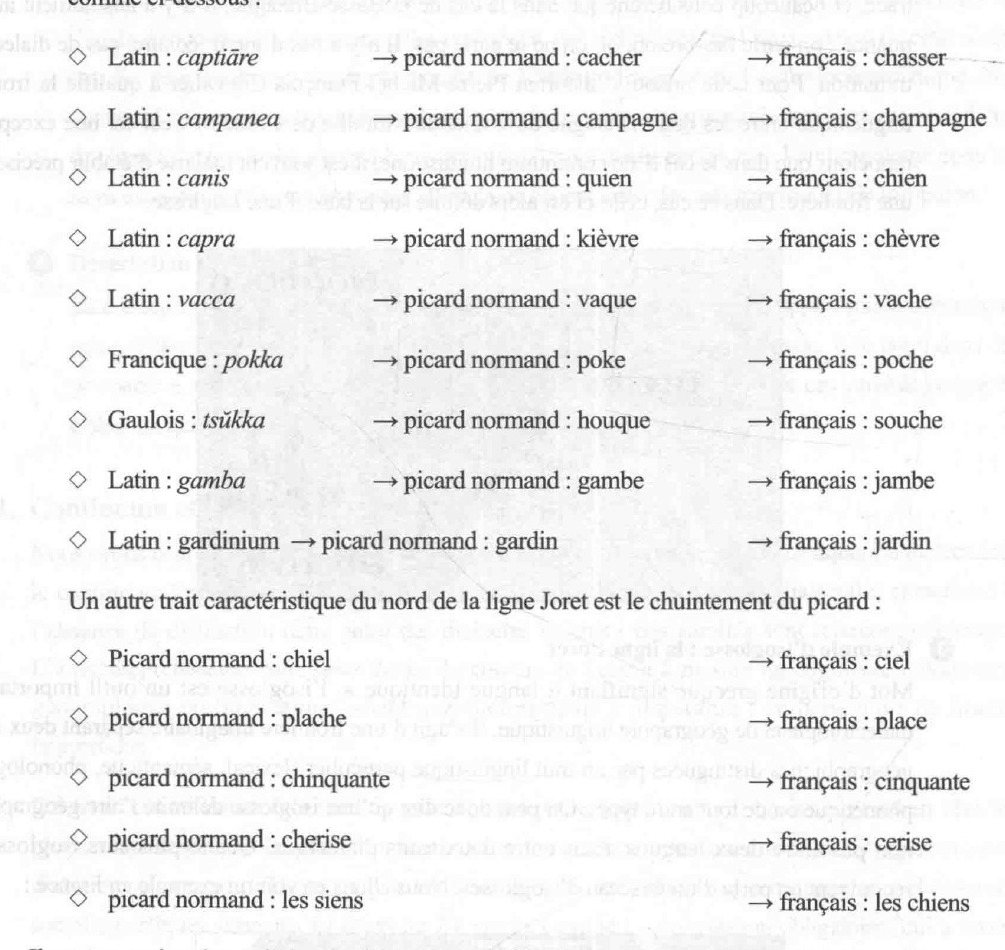
\includegraphics[width=.93\linewidth]{assets/ch13_joret_examples.jpg}
\end{center}

Il est temps à présent d’aborder l’interférence linguistique. Que se passe-t-il lorsque deux langues entrent en contact ?

\section{INTERFÉRENCES ENTRE SYSTÈMES LINGUISTIQUES}

\origpage{413}{399}

naissance a de nouveaux mots, mais a de véritables nouvelles langues.


\subsection{Langues vernaculaires et véhiculaires}

L’interférence linguistique est étroitement liée aux notions de langue vernaculaire et véhiculaire.


\minititle{Les langues vernaculaires}
Une langue vernaculaire est la langue locale communément parlée au sein d’une communauté. L’adjectif vernaculaire, dont le sens aujourd’hui est proche d’autochtone ou d’indigéne, vient du latin vernaculum. Ce mot désignait à l’époque tout ce qui était élevé, tissé, cultivé, confectionné à la maison, par opposition à ce que l’on se procurait par le commerce. C’est le grammairien romain Varron qui, le premier, a utilisé cet adjectif en linguistique.

\minititle{Les langues véhiculaires}
Une langue véhiculaire est une langue ou un dialecte servant de moyen de communication entre des populations de langues ou dialectes maternels différents. Il s’agit donc d’une langue tierce, différente des langues vernaculaires natives. Toutefois, une langue peut être à la fois véhiculaire et vernaculaire : c’est le cas par exemple de l’anglais, du français, et d’un certain nombre d’autres langues internationales, parlées à l’extérieur de leur espace national.

\subsection{Les langues de relation} Un sabir, une lingua franca, une koiné, un pidgin et un créole sont autant de langues de relations.


\minititle{Le sabir}
Les sabirs sont des langues véhiculaires et non maternelles nées du mélange de plusieurs langues vernaculaires. Le pionnier dans l’étude des sabirs a été le linguiste allemand Hugo Schuchardt (1842-1927) avec son article Die Lingua Franca (« La langue franque »), paru en 1909. Après lui, Dell Hymes et Uriel Weinreich ont consacré de nombreux travaux à ce qu’ils ont appelé « contact languages ».

Altération du mot saber qui en portugais, castillan, catalan et occitan signifie « savoir », le mot « sabir », apparu en 1852, désignait une langue utilisée dans le commerce pour communiquer en Afrique du Nord et au Moyen-Orient. Langage des ports de Méditerranée, il était fait d’un mélange de français, d’espagnol, de grec, d’italien et d’arabe. Étant destiné à usage commercial, le sabir était une langue d’appoint, un parler a minima au lexique pauvre, à la morphologie invariante et à la syntaxe primitive.


\minititle{La lingua franca}
Langue composite à base italienne, espagnole, comprenant de l’arabe, du provençal et du grec, la lingua franca (ou langue franque), est une langue parlée du Moyen âge jusqu’au 19e siècle dans l’ensemble du bassin méditerranéen. Dans son célèbre Dictionnaire universel (1690), le lexicographe Antoine Furetière (1619-1688) en a donné la définition suivante :

\origpage{414}{400}

Un jargon qu’on parle sur la mer Méditerranée, composé de français, d’italien, d’espagnol et d’autres langues, qui s’entend par tous les matelots et marchands de quelque nation qu’ ils soient.


L’adjectif franca s’explique par le fait qu’à l’époque, le mot « franc » désignait un Européen en général. Si elle était principalement parlée par les marins, les marchands, les explorateurs, les prisonniers, esclaves et populations déplacées de toutes origines, la lingua franca a aussi été utilisée par des ambassadeurs dans des pourparlers et négociations avec l’empire Ottoman et les états arabes : la proportion d’arabe qu'elle contenait donc a fortement augmenté avec le temps. En 1830, un manuel de lingua franca destiné aux militaires et aux administrateurs français des territoires arabes de la France, Langue franque, ou le petit mauresque, a été publié à Marseille. Dans un article de 1884, le général Louis Léon Faidherbe, administrateur colonial, présentait le sabir franco-arabe comme un moyen de favoriser l’emprise coloniale sur l’Afrique du Nord. Étant essentiellement utilitaire, la lingua franca a laissé très peu de traces écrites directes. Son vocabulaire était très limité, sa grammaire quasi-inexistante. Les verbes étaient utilisés à l’infinitif et sans aucune flexion. Ce n’est qu’au 17 siècle que sont apparues des distinctions rudimentaires de temps (passé, présent, futur).


\minititle{La koinè}

La koiné est, au sens propre, une forme de grec ancien qui a joué le rôle de langue commune (en grec ancien, koiné signifie « commune ») dans le monde hellénistique. La koiné grecque s’est développée comme dialecte commun entre les armées d’ Alexandre le Grand, différents dialectes grecs plus ou moins intercompréhensibles étant utilisés jusqu’alors. À la fin des conquêtes macédoniennes, la koiné était parlée depuis l’Égypte jusqu’aux frontières de l’Inde. Elle s’est imposée comme langue administrative et véhiculaire dans les zones sous influence hellénistique, avant d’entrer en concurrence avec le latin vulgaire. Ce dernier, dans l’Antiquité, servait de langue véhiculaire au sein des populations de la moitié occidentale de l’Empire romain en concurrence avec la koiné grecque dans la partie orientale.


\subsection{Les pidgins}


Entre les sabirs que je viens de présenter et les créoles que je vais présenter dans un instant, les linguistes distinguent la catégorie des pidgins, langues véhiculaires simplifiées créées sur le vocabulaire et certaines structures d’une langue de base, en général européenne (anglais, espagnol, français, néerlandais, portugais, etc.). Du point de vue sociolinguistique, un pidgin désigne une langue née de l’imitation de la langue d’une minorité dominante par un groupe linguistique dominé, dans le cas de la colonisation, par exemple.


\minititle{le pidgin anglo-chinois（洋泾浜英语）}

Le mot pidgin proviendrait de la corruption du mot « business » en pidgin anglo-chinois. Comme son nom l’indique, le pidgin anglo-chinois a pour base lexicale l’anglais basé sur un substrat chinois.

\origpage{415}{401}

\minititle{1. Contexte d’ apparition}

L’anglais est arrivé en Chine dans les années 1630, lorsque des commerçants anglais sont arrivés dans le sud du pays. Le pidgin anglo-chinois a d’abord été utilisé comme lingua franca dans les régions de Macao et du Guangdong (où les Anglais ont établi des ports de commerce en 1664) avant de prendre son essor à Shanghai dans les années 1830. L’anglais de « yangjing bang » tire son nom d’une ancienne petite crique à côté du Bund à Shanghai dans laquelle les travailleurs locaux utilisaient le pidgin pour échanger avec les étrangers anglophones. Depuis, la crique de Yang Jing a été comblée, et correspond aujourd’hui à la partie à l’est de la rue de Yan’an, la principale artère est-ouest de Shanghai. Le pidgin anglo-chinois a été utilisé jusqu’à la fin du 19e siècle avant d’être progressivement abandonné, les Chinois se tournant vers l’apprentissage de l’anglais standard.


\minititle{2. Traces dans le chinois moderne}

Si le pidgin anglo-chinois a disparu, la langue chinoise actuelle a conservé un grand nombre de mots qui en sont issus. En voici quelques exemples :


\begin{center}
\renewcommand{\arraystretch}{1.18}
\begin{tabularx}{.92\linewidth}{@{}XXX@{}}
马达 & 咖喱 & 雪茄\\
马赛克 & 阿司匹林 & 高尔夫\\
瓦斯 & 麦克风 & 华尔兹\\
吉普 & 沙发 & 夹克衫\\
摩托车 & 派队 & 车胎\\
柠檬 & 抬头 & 贝雷帽\\
土司 & 卡车 & 冰激凌\\
布丁 & 卡片 & 霓虹灯\\
三明治 & 酒吧 & 俱乐部\\
可可 & 沙丁鱼 & 维他命\\
\end{tabularx}
\end{center}

\minititle{Le pidgin camerounais : le camfranglais}


Quittons la Chine, direction l’Afrique. Le Cameroun, pays connu pour la grande diversité de ses langues (près de 250), a depuis longtemps adopté l’anglais et le français comme langues officielles. Toutefois, cette situation de diglossie étant très déséquilibrée, une nouvelle langue est apparue : le camfranglais.


\minititle{1. Contexte d’apparition}

Même si la plupart des habitants du Cameroun sont polyglottes et savent parler une ou plusieurs langues vernaculaires, ils sont soit francophones, soit anglophones, mais rarement les deux à la fois. Pour leur communication interethnique, les Camerounais ont longtemps utilisé des langues


\origpage{416}{402}

véhiculaires non officielles, comme le Pidgin anglais ou les langues locales. Dans les années 1970, une nouvelle langue est apparue : le camfranglais. Il s’agit d’une langue hybride, composée d’anglais, de français, et de langue locales Camerounaises. Parlé à l’origine par les jeunes lycéens et étudiants des grandes métropoles du Cameroun comme Douala ou Yaoundé, le camfranglais est de nos jours parlé dans tout le pays. Plus important, il est largement utilisé dans la littérature et dans les chansons populaires.


\minititle{2. Statut linguistique}

Dès sa naissance, le camfranglais a suscité de nombreuses controverses académiques quant a sa nature linguistique. Certains linguistes le considéraient comme un sociolecte jeune et hybride, sorte d’argot urbain, d’autres le considéraient comme un pidgin. Le camfranglais est certes né de l’interférence des langues locales Camerounaises avec les deux langues officielles du pays, mais son utilisation ne se borne plus seulement au domaine du commerce : utilisé dans la vie de tous les jours, il n’est donc plus un pidgin. Par ailleurs, même s’il est vrai que le camfranglais est apparu au départ comme une variété générationnelle, un parler des jeunes à la fonction cryptique, il s’est rapidement diffusé auprès d’une population plus âgée.


En 2014, le professeur Peter Wuteh Vakunta, auteur de Camfranglais, The Making of a New Language in Cameroonian Literature, réclamait la reconnaissance du camfranglais comme une langue indépendante. En voici quelques exemples de cette nouvelle langue :


Ex: On va all back au mboa (nous allons tous rentrer au pays). On go au school all les days (Nous allons à l’école tous les jours). Elle ne know pas mô comment on do ça (elle ne sait pas bien le faire). Je veux tra (je veux essayer).


Appris de nos jours comme langue maternelle, le camfranglais est une langue nationale mais n’a pas obtenu le statut de langue officielle, contrairement au bichlamar des îles Vanuatu.


\minititle{Le bichlamar des îles Vanuatu}


Le bichlamar est un pidgin à base lexicale anglaise parlé au Vanuatu, archipel situé dans l’Océan Pacifique qui compte environ cent cinq langues vernaculaires : on comprend donc la nécessité d’une langue véhiculaire. Depuis son indépendance en 1980, le bichlamar est devenu l’une des trois langues officielles de la République du Vanuatu, avec le français et l’anglais.


\minititle{1. Contexte d’apparition}

Le mot « bichlamar » vient du portugais bicho do mar, qui désigne en français l’holothurie (le concombre de mer). Le commerce de ce produit s’est d’abord fait avec les Malais, puis il s’est étendu dans le Pacifique-Sud. Au milieu du 19e siècle, des trafiquants sont allés les ramasser sur les récifs des îles mélanésiennes pour les revendre en Chine. La langue parlée entre ces navigateurs


\origpage{417}{403}

et les populations locales, un sabir à base d’anglais, constituait la toute première forme du futur bichlamar.


Dans la première moitié du 19e siècle, la Polynésie a été le lieu d’une importante activité de pêche à la baleine, et de nombreux autochtones ont été engagés pour travailler sur les bateaux de pêche. Comme ils venaient d’îles différentes, les membres de ces équipages utilisaient un pidgin pour communiquer entre eux.


Aux environs de 1860, de nouvelles plantations ont été développées en Australie : la canne à sucre, le coton et la coprah. Comme ces cultures réclamaient beaucoup de main d’œuvre, près de 50 000 habitants du Vanuatu ont été engagés dans les plantations. Ces travailleurs venaient d’îles différentes et parlaient donc des langues différentes : pour communiquer, ils utilisaient donc un pidgin.


C’est ce pidgin originel, de base lexicale anglaise mais conservant la syntaxe des langues mélanésiennes locales, qui, en évoluant, à donné naissance au bislama (bichlamar), mais aussi au tok pisin parlé aujourd’hui en Papouasie-Nouvelle-Guinée, au pijin des îles Salomon, que je vais présenter un peu plus bas. En 1910, le bichlamar, une fois stabilisé linguistiquement, a commencé à se répandre comme lingua franca dans tout l’archipel du Vanuatu.


\minititle{2. Statut linguistique}

Après avoir obtenu son indépendance de la France en 1980, la toute nouvelle République du Vanuatu a accordé au bichlamar le statut de langue officielle. En 1981, il est devenu langue liturgique lorsque les Églises de Vanuatu ont accepté de l’utiliser comme langue de communication avec les fidèles. Dans les deux zones urbaines du pays (Port-Vila et Santo), il est ainsi devenu la première langue de nombreux locuteurs qui ont cessé de parler leur langue d’origine. Nous reviendrons un peu plus bas sur ce processus appelé « créolisation ».


Le bichlamar garde néanmoins son statut de pidgin, c’est-à-dire de langue véhiculaire, dans les zones rurales du Vanuatu qui continuent encore aujourd’hui à parler les langues vernaculaires d'origine.


\minititle{3. Lexique en bichlamar}
Quand vous aurez lu lexique ci-dessous et constaté la grande simplicité du bichlamar, nul doute que vous regretterez d’avoir choisi d’étudier le français :
\begin{center}
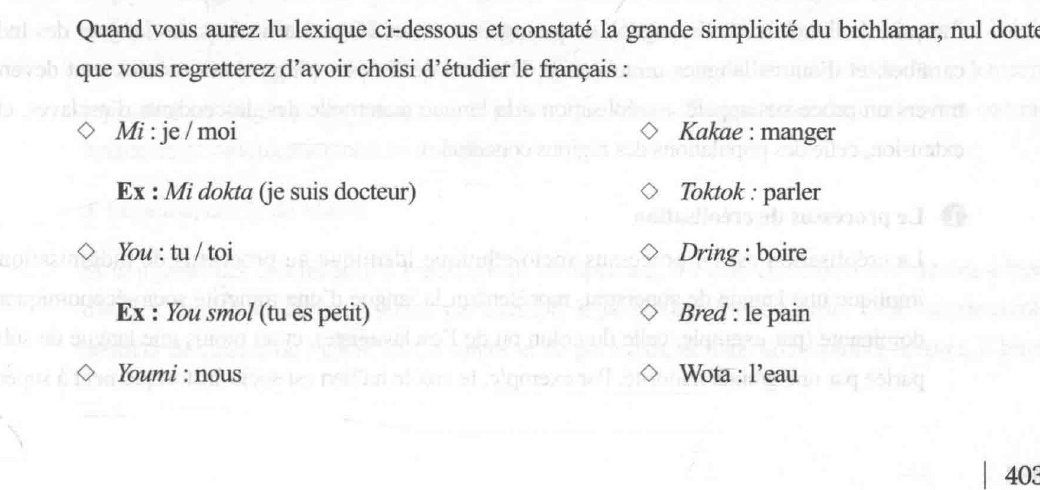
\includegraphics[width=.90\linewidth]{assets/ch13_bislama_lexicon_1.jpg}
\end{center}
\origpage{418}{404}
\begin{center}
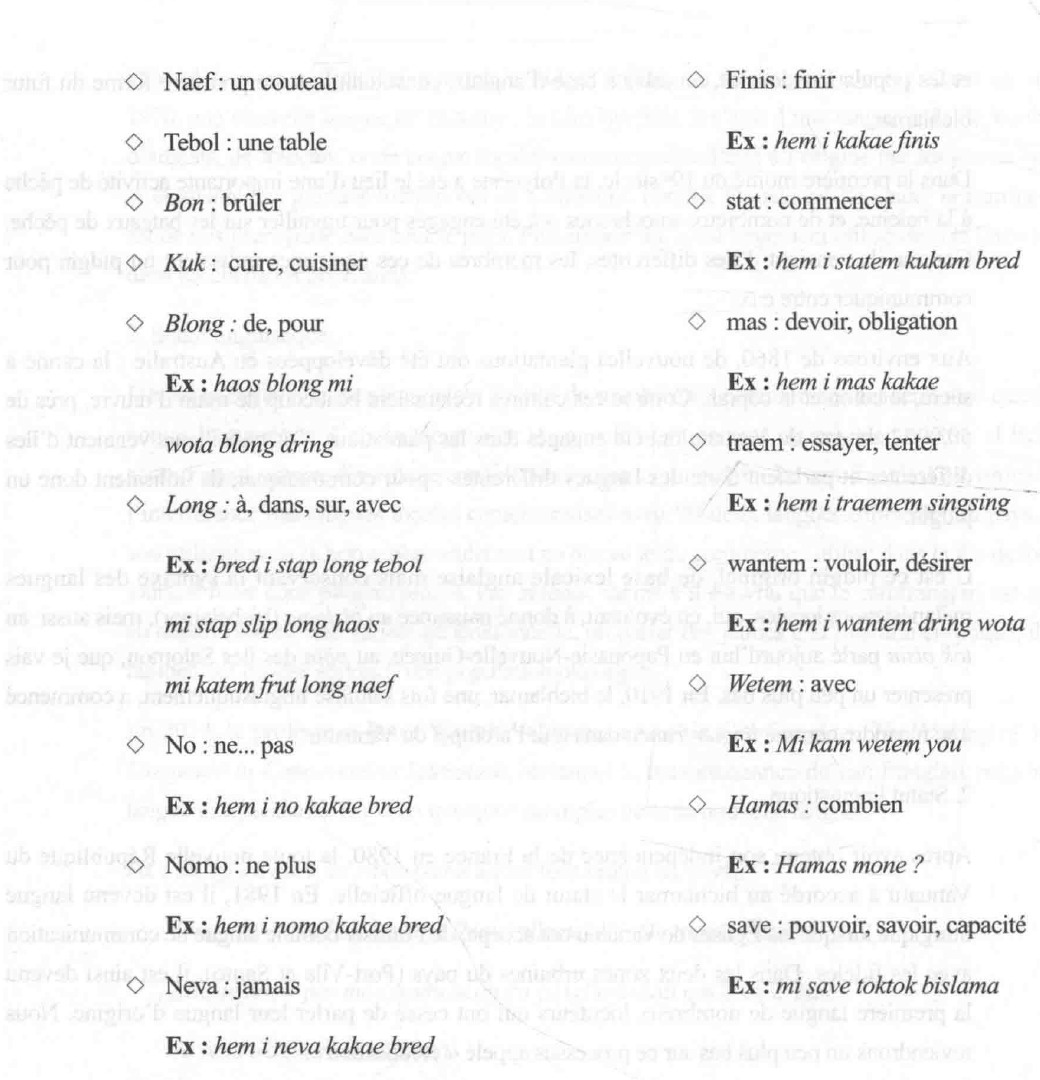
\includegraphics[width=.90\linewidth]{assets/ch13_bislama_lexicon_2.jpg}
\end{center}
L’hymne de la République du Vanuatu est intitulé « youmi, youmi,youmi ». Vous devriez pouvoir le traduire sans difficulté et donc pouvoir dire avec fierté : « mi save toktok bislama ».


\subsection{Les créoles}


Nés dans un contexte colonial et esclavagiste, les créoles sont des langues issues du contact du français, de l’anglais, de l’espagnol, du portugais avec les langues africaines, les langues des Indiens caraïbes, et d’autres langues minoritaires. D’abord de simples pidgins, ces créoles sont devenus à travers un processus appelé « créolisation » la langue maternelle des descendants d’esclaves, et par


extension, celle des populations des régions concernées.


\minititle{Le processus de créolisation}
La créolisation est un processus socio-ethnique identique au processus de pidginisation qui implique une langue de superstrat, représentant la langue d’une minorité socio-économiquement dominante (par exemple, celle du colon ou de l’esclavagiste), et au moins une langue de substrat parlée par une grande majorité. Par exemple, le créole haïtien est socio-historiquement à superstrat

\origpage{419}{405}

français (le français colonial). De même, le français parlé par les esclaves noirs aux Antilles, en Guyane, Réunion, île Maurice, Seychelles, Guadeloupe, à Madagascar, en Louisiane et dans l’océan Indien a donné respectivement naissance aux créoles antillais, guyanais, réunionnais, mauricien, etc.


\minititle{Différence entre pidgin et créole}


Du point de vue linguistique, on peut d’abord distinguer les pidgins et les créoles en fonction de leur niveau respectif de structuration et de complexité. Mais les linguistes considèrent surtout qu’un pidgin devient un créole dès lors qu’il devient la langue maternelle (vernaculaire) de la population.


Le pidgin, quant à lui, et pour rappel, est toujours véhiculaire et n’est utilisé que dans les relations entre des individus qui gardent chacun leur langue maternelle. Autre distinction couramment admise, le terme « pidgin » désigne les langues de contact issues de l’anglais, et le terme « créole » celles issues du français. Même si du point de vue linguistique cet emploi est incorrect, certains locuteurs de créoles continuent eux-mêmes d’utiliser le terme « pidgin » pour désigner leur langue, ce qui contribue à renforcer la confusion entre les deux termes.


\minititle{Exemples de langues créoles} Comme dans le cas des pidgins, il existe de nombreux créoles à base lexicale indo-européenne, notamment anglaise, française, portugaise et néerlandaise.


\minititle{1. Le tok pisin de Papouasie}

Le tok pisin est une des langues officielles de la Papouasie-Nouvelle-Guinée, avec l’anglais et le hiri motu (langue véhiculaire non maternelle). Comme son nom ne l’indique pas, le tok pisin est un créole (et non plus un pidgin) à base lexicale anglaise qui compte environ deux millions de locuteurs, dont à peu près 500 000 natifs. Ce créole est la langue la plus parlée parmi les 850 langues de ce territoire. Le tok pisin est utilisé par les médias, le gouvernement de Papouasie- Nouvelle-Guinée, et certaines écoles primaires enseignant en tok pisin.


\minititle{2. Le pijin des îles Salomon}

Le pijin (pidgin des Salomon) est la langue véhiculaire à base lexicale anglaise des îles Salomon, archipel comptant environ 80 langues vernaculaires. Comme le tok pisin, il est devenu un créole en devenant la langue maternelle pour des « pijinophones » et de leurs descendants. Il demeure cependant un pidgin pour ceux qui ne le parlent que comme langue seconde, c’est-à-dire comme langue de communication non maternelle.


\minititle{3. Le patoa, créole de Macao}

Si la plupart des créoles sont à base lexicale européenne, il existe également des créoles à base d’autres familles de langue, comme par exemple le patoa (créole) de Macao. Cette langue créole contient des traces de malais, de cantonais et de portugais, et dans une moindre mesure, d’hindi


\origpage{420}{406}
\section*{Exercices}
\addcontentsline{toc}{section}{Exercices — chapitre 13}
\begin{keybox}[I]
\textbf{Dans cet extrait de \textit{La Gloire de mon père} (1957), de Marcel Pagnol, pourquoi Marcel réécrit-il sa lettre ? Quel phénomène sociolinguistique cela illustre-t-il ?}

« Un jour en rentrant de l’école à midi, le petit Paul, penché sur la rampe, cria dans l’escalier sonore :

« On t’a écrit une lettre à la poste ! Il y a un timbre dessus ! »

J’escaladai les marches deux à deux, et la rampe vibrante sonna comme un harpe de bronze. Sur la table, près de mon assiette, une enveloppe jaune portait mon nom, tracé en lettres inégales sur une ligne retombante.

« Je parie, dit mon père, que ce sont des nouvelles de ton ami Lili. »

Je n’arrivai pas à ouvrir l’enveloppe, dont je déchirai tour à tour les quatre coins : mon père la prit, et de la pointe d’un couteau, en découpa le bord avec une habileté de chirurgien.

Il en tomba d’abord une feuille de sauge et une violette séchée. Sur trois feuilles d’un cahier d’écolier, avec une grosse écriture, dont les lignes ondulantes contournaient des taches d’encre, Lili me parlait.

Il ne fut pas facile de déchiffrer cette écriture que l’orthographe n’éclairait guère. Mais mon père, grand spécialiste, y parvint après quelques tâtonnements. Il dit ensuite :

« Il est heureux qu’il lui reste trois ans pour préparer le certificat d’étude ! »

Le lendemain, en sortant de l’école, j’allai au bureau de tabac, et j’achetai une très belle feuille de papier à lettre. Elle était décorée, en haut à gauche, par une hirondelle imprimée en relief, qui tenait dans son bec un télégramme.

Dans l’après-midi du jeudi, je composai longuement le brouillon de ma réponse. Je relus deux fois ma prose, et j’y apportai quelques corrections de détail ; puis armé d’une plume neuve, je la recopiai, un buvard sous la main et la langue entre les dents. Ma calligraphie fut soignée, et mon orthographe parfaite, car je vérifiai, au moyen du Petit Larousse, quelques mots douteux.

Le soir, je montrai mon ouvrage à mon père : il me fit ajouter quelques s, et barrer un t inutile, mais il me félicita, et déclara que c’était une belle lettre, ce qui remplit d’orgueil mon cher petit Paul. Le soir, dans mon lit, je relus le message de Lili, et son orthographe me parut si comique que je ne pus m’empêcher d’en rire. Mais je compris tout à coup que tant d’erreurs et de maladresses étaient le résultat de longues heures d’application, et d’un très grand effort d’amitié : alors, je me levai sans bruit sur mes pieds nus, j’allumai la lampe à pétrole, et j’apportai ma propre lettre, mon cahier et mon encrier sur la table de la cuisine.

Je commençai par arracher d’un coup sec, trois pages du cahier : j’obtins ainsi les dentelures irrégulières que je désirais. Alors, avec une vieille plume, je recopiai ma trop belle lettre.

Je supprimai au passage, les s paternels ; j’ajoutai quelques fautes d’orthographe, que je choisis parmi les siennes : les perdrots, batistin, la glue et le dézastre. Enfin, je pris soin d’émailler mon texte de quelques majuscules inopinées. Ce travail délicat dura deux heures, et je sentis que le sommeil me gagnait.

Pourtant, je relus sa lettre, puis la mienne. Il me sembla que c’était bien, mais qu’il manquait encore quelque chose : alors, avec le manche de mon porte-plume, je puisai une grosse goutte d’encre, et sur mon élégante signature, je laissai tomber cette larme noire : elle éclata comme un soleil. »
\end{keybox}

\origpage{421}{407}
\begin{keybox}[II]
\textbf{Réécrivez le dialogue ci-dessous en utilisant le registre de langue soutenu.}

A : Pas mal, cette teuf !\par
B : Mais mate un peu comme ils sont tous bien fringués ! Moi j’ai l’air d’un clodo !
\end{keybox}

\origpage{422}{408}
\section*{Pour aller plus loin}
\addcontentsline{toc}{section}{Pour aller plus loin — chapitre 13}
\begin{small}
\begin{description}[style=nextline,leftmargin=0pt,labelindent=0pt]
\item[BOYER (Henri).] \textit{Langues en conflit : Études sociolinguistiques.} L’Harmattan, 1991.
\item[CALVET (L-J.).] \textit{La Sociolinguistique.} Coll. « Que sais-je ? ». Paris, PUF, 2005.
\item[CALVET (L-J.).] \textit{Linguistique et colonialisme.} Payot, 1974.
\origpage{423}{409}
\item[FISHMAN (J.).] \textit{Sociolinguistics: a brief introduction.} Rowley, Newbury House, 1970.
\item[GUMPERZ (J.).] \textit{Engager la conversation : Introduction à la sociolinguistique interactionnelle.} Paris, Minuit, 1989.
\item[HAGÈGE (C.).] \textit{Halte à la mort des langues.} Paris, Éditions Odile Jacob, 2002.
\item[HAMERS (J.F.) \& BLANC (M.).] \textit{Bilingualité et bilinguisme.} Margada, Bruxelles, 1990.
\item[HYMES (D.).] \textit{Foundations in Sociolinguistics: An Ethnographic Approach.} Philadelphia, University of Pennsylvania Press, 1974.
\item[LABOV (W.).] \textit{Sociolinguistique.} Paris, Éditions de Minuit, 1976.
\item[LABOV (W.).] \textit{The Social Stratification of English in New York City Department Stores.} Washington, D.C., Center for Applied Linguistics, 1966.
\item[LIETTI (A.).] \textit{Pour une éducation bilingue : Guide de survie à l’usage des petits Européens.} Payot, 1994.
\item[MACKEY (W.).] \textit{Bilinguisme et contact des langues.} Klincksieck, 1977.
\item[MAILLARD (J.P.) \& DUVERGER (J.).] \textit{L’Enseignement bilingue aujourd’hui.} Albin Michel, 1996.
\item[MITFORD (N.).] \textit{Noblesse oblige: An Enquiry into the Identifiable Characteristics of the English Aristocracy.} London, Hamish Hamilton, 1956.
\item[MITFORD (N.).] \textit{Snobisme et voyages.} Stock, 1964.
\item[ROSS (A.).] \textit{How to pronounce it.} London, Hamish Hamilton, 1970.
\item[ROSS (A.).] \textit{Linguistic class-indicators in present-day English.} Helsinki, Neuphilologische Mitteilungen, 1954.
\item[WEINREICH (U.).] \textit{Languages in contact: Findings and problems.} Mouton, 1968.
\end{description}
\end{small}

\section*{Glossaire}
\addcontentsline{toc}{section}{Glossaire — chapitre 13}
\gloss{alternance codique (code-switching)}{混合代码}{混合使用两种代码或语言，通常在同一话题内。这种情况在双语或多语环境中非常普遍。}
\gloss{bilinguisme}{双语制}{个人或群体使用至少两种语言。}
\gloss{continuum linguistique}{语言变体连续统}{一系列语言变体。虽然人们常认为一种语言可分为若干独立地区方言或社会方言，但它们之间往往没有明确界限，而是一种方言到另一种方言之间构成了一个连续统。}
\origpage{424}{410}
\gloss{créole}{克里奥语}{已成为某一群体的本族语的洋泾浜语，用于该群体部分或全部的日常交际，一般克里奥语的句子结构和词汇量要比洋泾浜语复杂得多。}
\gloss{dialectologie}{方言学}{关于语言地区变异的研究，通常注意不同方言表示同一物体的不同单词或同一单词在不同方言里的不同发音。}
\gloss{diglossie}{双言制，双言现象}{一个团体内同时存在两种语言或语言的两种变体，各用于不同的目的。}
\gloss{frontière linguistique}{语言界限，语言边境}{区别两种不同方言或语言间的虚构的地理界限。}
\gloss{hypercorrection}{矫枉过正；过分庄重}{语言运用中规则的泛化，或是指说话时由于企图表现得有教养，替换了一个本身正确形式时所出现的单词、发音或其他语言特征的错误使用。}
\gloss{isoglosse}{同言线}{语言地图上，标记某一语言特征使用范围的边界。通常认为，一束同言线表示一种方言的边境的存在。}
\gloss{multilinguisme}{多语制}{个人或群体如某一地区或国家的居民使用三种或三种以上的语言。}
\gloss{pidgin}{洋泾浜语}{操不同语言的群体在经常相互交际的过程中作为接触语言而发展起来的一种语言。}
\gloss{plurilinguisme}{多种语言的使用；使用多种语言的能力}{\emph{原书此词条仅列词头与中文释义，未见随后定义正文。}\ednote{底本第410页在 plurilinguisme 后直接进入 sociolinguistique 词条，故此处不以本章前文定义补写缺失内容。}}
\gloss{sociolinguistique}{社会语言学}{联系社会因素，即社会阶级、教育水平、教育类型、年龄、性别、种族等来研究语言的学科。}
\gloss{variation linguistique}{语言变异}{一种语言中发音、语法或词汇选择等方面的差异。}
